\documentclass[11pt,oneside]{article}

\usepackage[a4paper,margin=26mm,headheight=15pt]{geometry}
\usepackage[T1]{fontenc}
\usepackage[utf8]{inputenc}
\IfFileExists{libertinus.sty}{\usepackage{libertinus}}{\usepackage{lmodern}}
\usepackage{microtype}
\usepackage{amsmath,amssymb,amsthm,mathtools,mathrsfs,bm}
\usepackage{booktabs,longtable,tabularx,array,multirow}
\usepackage{graphicx}
\usepackage{xcolor}
\usepackage{enumitem}
\usepackage{fancyhdr}
\usepackage{titlesec}
\usepackage{xurl}
\usepackage{listings}
\usepackage{hyperref}
\usepackage[nameinlink,noabbrev]{cleveref}

\definecolor{linkblue}{RGB}{24,72,124}
\definecolor{deepgreen}{RGB}{23,102,69}
\definecolor{deepred}{RGB}{140,42,42}
\definecolor{shadegray}{RGB}{246,247,249}
\definecolor{rulegray}{RGB}{195,201,208}
\hypersetup{
  colorlinks=true,
  linkcolor=linkblue,
  citecolor=deepgreen,
  urlcolor=linkblue,
  pdftitle={Exponent-Sequence and Newton-Basis Frontiers for the Fabius--Rvachev System},
  pdfauthor={OpenAI GPT-5.6 Pro},
  pdfsubject={New spectral, cumulant, q-Richardson, automatic-sequence, Newton-basis, and endpoint results},
  pdfkeywords={Fabius function, inverse Fabius function, Rvachev up-function, Thue-Morse, q-binomial, Richardson extrapolation, Bell polynomial, Bernoulli polynomial, Lambert W}
}

\pagestyle{fancy}
\fancyhf{}
\fancyhead[L]{\small Exponent-sequence frontiers}
\fancyhead[R]{\small Fabius--Rvachev system}
\fancyfoot[C]{\thepage}
\renewcommand{\headrulewidth}{0.4pt}

\titleformat{\section}{\Large\bfseries\color{linkblue}}{\thesection}{0.72em}{}
\titleformat{\subsection}{\large\bfseries\color{linkblue}}{\thesubsection}{0.65em}{}
\titleformat{\subsubsection}{\normalsize\bfseries\color{deepgreen}}{\thesubsubsection}{0.58em}{}
\setcounter{tocdepth}{2}
\setcounter{secnumdepth}{3}
\numberwithin{equation}{section}
\allowdisplaybreaks[3]
\setlength{\emergencystretch}{3em}
\setlist[itemize]{leftmargin=2em,itemsep=0.25em,topsep=0.45em}
\setlist[enumerate]{leftmargin=2.3em,itemsep=0.25em,topsep=0.45em}

\newtheorem{theorem}{Theorem}[section]
\newtheorem{proposition}[theorem]{Proposition}
\newtheorem{lemma}[theorem]{Lemma}
\newtheorem{corollary}[theorem]{Corollary}
\newtheorem{conjecture}[theorem]{Conjecture}
\newtheorem{problem}[theorem]{Open problem}
\theoremstyle{definition}
\newtheorem{definition}[theorem]{Definition}
\newtheorem{algorithm}[theorem]{Algorithm}
\newtheorem{example}[theorem]{Example}
\theoremstyle{remark}
\newtheorem{remark}[theorem]{Remark}
\newtheorem{warning}[theorem]{Warning}

\newcommand{\R}{\mathbb R}
\newcommand{\C}{\mathbb C}
\newcommand{\Q}{\mathbb Q}
\newcommand{\N}{\mathbb N}
\newcommand{\Z}{\mathbb Z}
\newcommand{\E}{\mathbb E}
\newcommand{\Prob}{\mathbb P}
\newcommand{\Var}{\operatorname{Var}}
\newcommand{\Cov}{\operatorname{Cov}}
\newcommand{\Law}{\operatorname{Law}}
\newcommand{\Up}{\operatorname{up}}
\newcommand{\sinc}{\operatorname{sinc}}
\newcommand{\sgn}{\operatorname{sgn}}
\newcommand{\ord}{\operatorname{ord}}
\newcommand{\Res}{\operatorname*{Res}}
\newcommand{\supp}{\operatorname{supp}}
\newcommand{\vtwo}{\nu_2}
\newcommand{\wt}{s_2}
\newcommand{\dd}{\,\mathrm d}
\newcommand{\e}{\mathrm e}
\newcommand{\ii}{\mathrm i}
\newcommand{\bigO}{\mathcal O}
\newcommand{\smallo}{o}
\newcommand{\qbinom}[3]{\genfrac{[}{]}{0pt}{}{#1}{#2}_{#3}}
\newcommand{\fall}[2]{#1^{\underline{#2}}}
\newcommand{\repo}{\textsc{ProveIt}}
\newcommand{\statusproved}{\textcolor{deepgreen}{\textbf{proved here}}}
\newcommand{\statusderived}{\textcolor{linkblue}{\textbf{derived from audited corpus theorems}}}
\newcommand{\statusopen}{\textcolor{deepred}{\textbf{conjectural/open}}}
\newcommand{\NormalCDF}{\Phi_{\!G}}
\newcommand{\NormalSurv}{\overline{\Phi}_{\!G}}
\newcommand{\Bell}{\mathcal B}
\newcommand{\Agen}{\mathcal A}
\newcommand{\Zspec}{\mathcal Z}
\newcommand{\Mellin}{\mathcal M}

\newenvironment{statusbox}[1]{%
  \par\medskip\noindent\begin{center}\begin{minipage}{0.94\textwidth}%
  \color{linkblue}\hrule\vspace{0.65em}%
  \color{black}\textbf{\color{linkblue}#1.}\ }{%
  \par\vspace{0.65em}\color{linkblue}\hrule
  \end{minipage}\end{center}\medskip}

\newenvironment{resultbox}[1]{%
  \par\medskip\noindent\begin{center}\begin{minipage}{0.94\textwidth}%
  \color{deepgreen}\hrule\vspace{0.65em}%
  \color{black}\textbf{\color{deepgreen}#1.}\ }{%
  \par\vspace{0.65em}\color{deepgreen}\hrule
  \end{minipage}\end{center}\medskip}

\lstdefinestyle{python}{
  language=Python,
  basicstyle=\ttfamily\small,
  backgroundcolor=\color{shadegray},
  frame=single,
  rulecolor=\color{rulegray},
  columns=fullflexible,
  breaklines=true,
  keepspaces=true,
  showstringspaces=false,
  keywordstyle=\color{linkblue}\bfseries,
  commentstyle=\color{deepgreen},
  stringstyle=\color{deepred}
}

\title{\bfseries Exponent-Sequence and Newton-Basis Frontiers\\[0.2em]
for the Fabius--Rvachev System\\[0.55em]
\large A universal spectral--cumulant dictionary, certified $q$-Richardson tomography,\\
positive-definite Pascal quotients, automatic lobe signs, and Gaussian boundary layers}
\author{Frontier research report based on the complete recursive \texttt{*.tex} corpus under\\
\small\path{Analysis/FabiusFunction/docs}}
\date{Pinned repository snapshot: 27 August 2026\\
\small commit \texttt{32d6d36c51d803289e6d6a0dc0c37753766eba47}}

\begin{document}
\maketitle

\begin{abstract}
The audited \repo{} corpus already contains the classical Fabius and Rvachev functions,
exact dyadic arithmetic, the full Thue--Morse formula atlas, Gaussian $q$-binomial
interpolation, all-orders endpoint expansions, lower-branch Lambert-$W$ coordinates,
Bell- and Bernoulli-polynomial coefficient calculus, sharp Fourier decay, the integer-zero
spectrum of the Rvachev transform, a spectral determinant, rational arithmetic rays,
half-integer quadrature identities, logarithmic $q$-Richardson acceleration, and a
Pascal-weighted hierarchy of compactly supported densities.  This report avoids repackaging
those results.  Instead it identifies a single master object that contains them as special
coordinates and exposes several new deductions.

For a nonnegative integer exponent sequence $a=(a_h)_{h\ge0}$ with
$A(1/2)<\infty$, where $A(q)=\sum_{h\ge0}a_hq^h$, define
\[
 \Phi_a(z)=\prod_{h\ge0}\sinc\!\left(\frac{z}{2^h}\right)^{a_h},
 \qquad \sinc z=\frac{\sin\pi z}{\pi z}.
\]
It is the characteristic function of an explicit compactly supported convolution of
uniform variables.  We prove a universal dictionary in which the same generating function
$A$ controls: the integer-zero multiplicity
$m_a(n)=\sum_{h\le\nu_2(n)}a_h$; the spectral zeta
$\mathcal Z_a(s)=\zeta(s)A(2^{-s})$; every even cumulant
$\kappa_{2j}=B_{2j}A(4^{-j})/(2j)$; the Fourier-lobe sign; exact digital zero counts;
and the order of Prouhet cancellation of each finite sign block.  The zero divisor, the
spectral zeta quotient, and the complete even-cumulant sequence each determine $a$ uniquely.

The cumulant samples $A(4^{-m})$ admit a new exact reconstruction mechanism.  Lagrange
extrapolation at geometric nodes has Gaussian-$q$-binomial weights, an exact transformed
series, fixed alternating sign, bounded $\ell^1$ condition number, and certified integer
brackets.  Thus Richardson extrapolation becomes a stable tomography algorithm for the
hidden dyadic exponent sequence.

For polynomial exponent sequences, the Newton expansion
$P(h)=\sum c_r\binom hr$ gives the finite factorization
$\Phi_P=\prod_r\Phi_{r+1}^{c_r}$ through the audited Pascal--Rvachev hierarchy.  Negative
Newton coefficients are allowed: whenever $P(h)\ge0$ on the nonnegative integers, the
resulting alternating quotient is nevertheless entire and positive definite.  The even
family
\[
 P_d(h)=\binom{h-1}{d},\qquad d=0,2,4,\ldots,
\]
is especially striking.  It satisfies
\[
 \Psi_d(z)=\sinc(z)\Phi_{d+1}(z/2)
 =\prod_{r=0}^d\Phi_{r+1}(z)^{(-1)^{d-r}},
\]
has support $[-1,1]$, zero multiplicity
$1+\binom{\nu_2(n)}{d+1}$, and converges in total variation to the uniform law.  Its
transition across the two discontinuities of the limiting box density has a Gaussian
boundary layer with an explicit Berry--Esseen rate.  For $d=2$ this supplies the concrete
positive-definite quotient $\Phi_1\Phi_3/\Phi_2$.

Finally, a Mellin-reflection identity relates the endpoint Laplace transform directly to
the reflected spectral zeta.  For polynomial weights it explains the complete hierarchy
of logarithmic powers and periodic coefficients, gives a generalized lower-Lambert saddle,
and yields the leading inverse-endpoint law.  Reasonable conjectures and a detailed research
and Lean-formalization program conclude the report.  Numerical experiments were independently
implemented at high precision; the commented Python source and generated data accompany the
paper.
\end{abstract}

\tableofcontents
\clearpage

\section{Audit boundary, source stratification, and novelty discipline}
\label{sec:audit}

\subsection{Pinned corpus}

The repository changed several times on the audit date, so the source boundary is the exact
commit printed on the title page.  Its recursive documentation tree contains 67 distinct
\texttt{.tex} paths: five living synthesis/reference documents, thirty-two frozen historical
sources, twenty-three active frontier drafts (including twelve Fourier-decay dossiers), and
seven transcribed or corrected source papers.  Every path is listed in
\cref{app:inventory}.  Historical revisions were read as mathematical lineages rather than
as independent evidence; the archive's provenance ledger identifies what was superseded,
merged, or deliberately frozen.

The living primary exposition separates the bounded distribution function, the compactly
supported Rvachev bump, and the signed global extension, and confines itself to claims with
matching Lean declarations.  The consolidated frontier volume and its current descendants
contain the non-formalized but mathematically developed material.  In particular, the audit
treated the following as prior art rather than as discoveries of this report:
\begin{itemize}
\item the integer zero set and multiplicity $1+\nu_2(n)$ of the classical Rvachev transform;
\item its spectral determinant, spectral zeta, heat trace, local zero jets, and symmetric
      $q$-integer deformation;
\item the full signed Thue--Morse formula atlas, Prouhet cancellation, Mahler products,
      rarefied sums, Mellin--Dirichlet theory, and automatic-sequence machinery;
\item exact dyadic values of $F$, half-base $q$-Pochhammer and Gaussian-binomial formulas,
      Lagrange interpolation, and several existing Richardson transforms;
\item the corrected lower-Lambert endpoint expansion, its nonconstant periodic factor,
      all-order Bell-polynomial coefficient construction, and the inverse Fabius expansion;
\item sharp geometric, arithmetic, metric, and envelope results for the infinite sinc product;
\item cyclotomic rational rays, half-integer spectral identities, exact zero jets, and the
      Pascal hierarchy
      $\Phi_r(z)=\prod_h\sinc(z/2^h)^{\binom h{r-1}}$;
\item logarithmic $q$-Richardson acceleration of truncated sinc products and phase-locked
      Richardson extraction of the endpoint periodic term;
\item positive Gaussian and Lobatto tail quadrature, exact ordinary-prefix error laws,
      generalized gamma-convolution duality, and the existing Gaussian rank limit for the
      Pascal hierarchy.
\end{itemize}

\subsection{What is new relative to the pinned tree}

Targeted path, phrase, and formula searches found no counterpart of the following theorem
package in the audited snapshot:
\begin{enumerate}
\item the arbitrary nonnegative exponent-sequence monoid and its single generating-function
      dictionary for zero spectra, cumulants, digital signs, and endpoint Mellin transforms;
\item exact digital zero-count defects and generalized Prouhet order for an arbitrary
      exponent parity word, including the first surviving power moment;
\item equivalence and constructive recovery of the exponent sequence from either the zero
      divisor or all even cumulants;
\item certified Gaussian-$q$-binomial Richardson tomography of the exponent coefficients;
\item the finite-refinement-rank classification by rational ordinary generating functions;
\item the Newton-basis factorization of every nonnegative integer-valued polynomial weight,
      including positive-definite alternating quotients of Pascal transforms;
\item the normalized family $P_d(h)=\binom{h-1}{d}$ for even $d$, its sparse zero spectrum,
      automatic sign selector, exact total-variation law, and Gaussian boundary layer;
\item the general spectral--endpoint Mellin reflection formula
      $\Mellin[\log L_a](w)=-\Gamma(w)\zeta(w+1)\mathcal Z_a(-w)/\zeta(-w)$;
\item the polynomial-weight universality theorem and its generalized Lambert-$W_{-1}$
      endpoint coordinate.
\end{enumerate}

A targeted external search located the classical ingredients separately---the original
Fabius--Rvachev analysis and arithmetic, lacunary Thue--Morse products, automatic sequences,
Berry--Esseen bounds, rational and integer-valued generating functions, Mellin harmonic sums,
exponential Tauberian transfer, and Lambert inversion
\cite{arias1982,arias2017,aistleitner2015,toth2022,alloucheShallit,petrov1995,
stanley1997,flajolet1995,debruijn1959,corless1996}---but not this combined classification.
Accordingly, ``new'' below always means new to the pinned corpus and apparently nonstandard;
it is not an assertion of exhaustive worldwide priority.

\begin{statusbox}{Proof-status convention}
Results explicitly labeled \statusproved{} are proved in this manuscript.  Results labeled
\statusderived{} use a theorem already developed in the audited frontier corpus (most often
the sharp Pascal-hierarchy Fourier or endpoint asymptotic) and then add a new deduction.
Items labeled \statusopen{} are conjectures or proposed programs.  At the pinned snapshot,
none of the new results was represented as already formalized in Lean.  There is one explicit
post-snapshot exception: source checkpoint
\path{1e761ed77583e9870ceeaeb2c74ac824094f0f3f} formalizes the
denominator-free principal specialization and complete positive-degree geometric-moment
identities used in \cref{lem:q-weights}.  It does not formalize this report's exponent-sequence
classification, transformed analytic series, sign-certified remainder, tomography, or
asymptotic applications.
\end{statusbox}

\section{The exponent-sequence convolution monoid}
\label{sec:master}

\subsection{Admissible sequences}

Throughout, the normalized entire sinc is
\begin{equation}
 \sinc z=\frac{\sin\pi z}{\pi z},\qquad \sinc0=1.
 \label{eq:sinc-normalized}
\end{equation}
It is the Fourier transform, under the kernel $\e^{-2\pi\ii zx}$, of the uniform
probability density on $[-1/2,1/2]$.

\begin{definition}[Admissible exponent sequence]
A sequence $a=(a_h)_{h\ge0}$ is \emph{admissible} if
\[
 a_h\in\N_0,
 \qquad
 A(q):=\sum_{h\ge0}a_hq^h,
 \qquad
 A(1/2)<\infty.
\]
Its generalized Rvachev transform is
\begin{equation}
 \Phi_a(z)=\prod_{h=0}^{\infty}
 \sinc\!\left(\frac{z}{2^h}\right)^{a_h}.
 \label{eq:Phi-a}
\end{equation}
\end{definition}

For each $h$ and $1\le j\le a_h$, let $U_{h,j}$ be independent and uniform on
$[-1/2,1/2]$, and put
\begin{equation}
 X_a=\sum_{h\ge0}\sum_{j=1}^{a_h}2^{-h}U_{h,j},
 \qquad
 R_a=\frac12A(1/2).
 \label{eq:X-a}
\end{equation}
Absolute convergence is deterministic because the sum of the radii is $R_a$.

\begin{theorem}[Probability, analyticity, support, and convolution]
\label{thm:master-probability}
For every admissible $a$:
\begin{enumerate}
\item $X_a$ is supported on $[-R_a,R_a]$ and has characteristic function $\Phi_a$;
\item the product in \eqref{eq:Phi-a} converges locally uniformly on $\C$, hence is entire;
\item $\Phi_{a+b}=\Phi_a\Phi_b$, and the corresponding probability law is the convolution
      of the laws for $a$ and $b$;
\item if $\sum_ha_h=\infty$, then $X_a$ has a compactly supported $C^\infty$ density;
      if only finitely many $a_h$ are nonzero, its law is a finite uniform box spline.
\end{enumerate}
All four assertions are \statusproved.
\end{theorem}

\begin{proof}
Independence gives the finite-prefix characteristic products.  The variables are bounded and
$\sum_{h,j}|2^{-h}U_{h,j}|\le R_a$, so the finite sums converge almost surely and in every
$L^p$, and their characteristic functions converge to that of $X_a$.

Locally, $\log\sinc w=\bigO(w^2)$.  Since
$\sum_ha_h4^{-h}=A(1/4)<\infty$, the logarithms of the factors converge normally on compact
sets avoiding a harmless choice of local branch; standard infinite-product theory then gives
an entire limit.  Addition of exponent sequences is multiplication of products, which is
exactly convolution of independent sums.

If infinitely many individual factors occur, fix $M$ of them.  On the real axis,
$|\sinc(\xi/2^h)|\le\min(1,2^h/(\pi|\xi|))$.  The chosen $M$ factors give
$|\Phi_a(\xi)|\le C_M(1+|\xi|)^{-M}$, while all remaining factors have modulus at most one.
Thus $\Phi_a$ is rapidly decreasing; Fourier inversion gives a $C^\infty$ density.  With
finitely many factors one obtains a finite convolution of interval densities, hence a box
spline.
\end{proof}

\begin{remark}
The classical Rvachev transform corresponds to $a_h\equiv1$.  The audited Pascal hierarchy
corresponds to $a_h=\binom h{r-1}$.  The point of \cref{thm:master-probability} is not merely
that both products exist, but that the collection of all such laws is a commutative
convolution monoid whose algebra is the coefficientwise additive monoid of exponent
sequences.
\end{remark}

\section{Integer zeros, spectral zeta, digital defects, and lobe signs}
\label{sec:spectrum}

\subsection{The universal zero-divisor formula}

Euler's product for the normalized sinc gives
\[
 \sinc z=\prod_{k\ge1}\left(1-\frac{z^2}{k^2}\right).
\]
An integer $n\ne0$ is a zero of the scale-$h$ factor precisely when $2^h\mid n$.
This immediately yields the following master theorem.

\begin{theorem}[Zero divisor and spectral zeta]
\label{thm:zero-zeta}
Let $a$ be admissible and define
\begin{equation}
 m_a(n)=\sum_{h=0}^{\vtwo(n)}a_h,
 \qquad n\ge1.
 \label{eq:m-a}
\end{equation}
Then
\begin{equation}
 \boxed{\quad
 \Phi_a(z)=\prod_{n\ge1}\left(1-\frac{z^2}{n^2}\right)^{m_a(n)}
 \quad}
 \label{eq:canonical-a}
\end{equation}
with locally uniform convergence.  In particular,
$\ord_{z=\pm n}\Phi_a=m_a(n)$.  For $\Re s>1$,
\begin{equation}
 \boxed{\quad
 \Zspec_a(s):=\sum_{n\ge1}\frac{m_a(n)}{n^s}
 =\zeta(s)A(2^{-s}).
 \quad}
 \label{eq:zeta-a}
\end{equation}
Both statements are \statusproved.
\end{theorem}

\begin{proof}
The scale-$h$ sinc contributes one zero at $n$ for every representation $n=2^hk$ with
$k\ge1$, and it occurs with multiplicity $a_h$.  Summing over $h\le\vtwo(n)$ gives
\eqref{eq:m-a}.  Moreover
\[
 \sum_{n\ge1}\frac{m_a(n)}{n^2}
 =\sum_{h\ge0}a_h\sum_{k\ge1}\frac1{(2^hk)^2}
 =\zeta(2)A(1/4)<\infty,
\]
so the genus-zero canonical product converges normally.  The same rearrangement for
$\Re s>1$ gives
\[
 \sum_{n\ge1}\frac1{n^s}\sum_{2^h\mid n}a_h
 =\sum_{h\ge0}a_h2^{-hs}\zeta(s).
\]
\end{proof}

\begin{resultbox}{Spectral--probabilistic dual use of $A$}
The spectral side samples $A$ at $2^{-s}$, while the probability side will sample it at
$4^{-j}$.  The entire zero divisor and every even cumulant are therefore two transforms of
one coefficient sequence, not merely analogous formulas.
\end{resultbox}

\subsection{Exact counting and a generalized digital defect}

Let
\begin{equation}
 M_a(N)=\sum_{n=1}^{N}m_a(n).
 \label{eq:M-a}
\end{equation}
For $N=\sum_{j\ge0}b_j(N)2^j$, define the tail weights
\begin{equation}
 \tau_j(a)=\sum_{k\ge1}a_{j+k}2^{-k}.
 \label{eq:tau-j}
\end{equation}

\begin{theorem}[Exact zero count and digit defect]
\label{thm:digital-count}
For every positive integer $N$,
\begin{align}
 M_a(N)
 &=\sum_{h\ge0}a_h\left\lfloor\frac{N}{2^h}\right\rfloor,
 \label{eq:M-floor}\\
 &=N A(1/2)-\rho_a(N),
 \qquad
 \rho_a(N)=\sum_{h\ge0}a_h\left\{\frac{N}{2^h}\right\},
 \label{eq:M-defect}\\
 &=N A(1/2)-\sum_{j\ge0}b_j(N)\tau_j(a).
 \label{eq:M-bit}
\end{align}
This is \statusproved.
\end{theorem}

\begin{proof}
Count the multiples of $2^h$ among $1,\ldots,N$ and sum their contributions $a_h$.
Subtracting the fractional parts from $N\sum_ha_h2^{-h}$ gives \eqref{eq:M-defect}.
Finally,
\[
 \left\{\frac{N}{2^h}\right\}
 =\sum_{j=0}^{h-1}b_j(N)2^{j-h};
\]
absolute convergence permits exchanging the sums and yields \eqref{eq:M-bit}.
\end{proof}

For $a_h\equiv1$, one has $A(1/2)=2$ and $\tau_j=1$, recovering the audited identity
$M_a(N)=2N-s_2(N)$.  For general $a$, the ordinary binary weight is replaced by a weighted
suffix transform of the exponent sequence.

\subsection{Lobe signs and generalized Thue--Morse characters}

For $x\in(N,N+1)$, every canonical-product factor with index $n\le N$ is negative and all
remaining factors are positive.  Hence
\begin{equation}
 \sgn\Phi_a(x)=(-1)^{M_a(N)}.
 \label{eq:lobe-sign-count}
\end{equation}
Modulo two,
$\lfloor N/2^h\rfloor\equiv b_h(N)$, so the sign is a digit character.

\begin{theorem}[Generalized lobe sign]
\label{thm:lobe-sign}
Put $\bar a_h=a_h\bmod2$ and
\begin{equation}
 \varepsilon_a(N)=(-1)^{\sum_{h\ge0}\bar a_hb_h(N)}.
 \label{eq:epsilon-a}
\end{equation}
Then, away from the integer zeros,
\begin{equation}
 \boxed{\qquad \sgn\Phi_a(x)=\varepsilon_a(\lfloor x\rfloor).\qquad}
 \label{eq:sign-master}
\end{equation}
Moreover $\varepsilon_a$ is a $2$-automatic sequence if and only if the parity word
$(\bar a_h)_{h\ge0}$ is eventually periodic.  Both statements are \statusproved.
\end{theorem}

\begin{proof}
The sign formula follows from \eqref{eq:lobe-sign-count}, \eqref{eq:M-floor}, and reduction
modulo two.  For the automaticity criterion, let $S$ denote the left shift of the parity
word.  If $0\le r<2^k$, binary concatenation gives
\begin{equation}
 \varepsilon_a(2^kn+r)=\varepsilon_a(r)\varepsilon_{S^ka}(n).
 \label{eq:kernel-shift}
\end{equation}
Thus an eventually periodic parity word has only finitely many shifts and therefore gives a
finite $2$-kernel.  Conversely, equality of two shifted sign sequences forces equality of
the corresponding shifted parity words, because
$\varepsilon_{S^ka}(2^j)=(-1)^{\bar a_{k+j}}$.  A finite $2$-kernel therefore implies a
finite shift orbit of the parity word, which is equivalent to eventual periodicity.  This is
the present Walsh-character specialization of the standard finite-kernel characterization
of automatic sequences \cite{alloucheShallit}.
\end{proof}

\subsection{Finite sign products and exact Prouhet order}

For $L\ge0$, let
\begin{equation}
 O_L(a)=\{0\le h<L:a_h\ \text{is odd}\},
 \qquad \omega_L(a)=|O_L(a)|.
 \label{eq:O-omega}
\end{equation}

\begin{theorem}[Generalized Prouhet block]
\label{thm:general-prouhet}
The length-$2^L$ sign polynomial factors as
\begin{equation}
 T_{a,L}(z):=\sum_{n=0}^{2^L-1}\varepsilon_a(n)z^n
 =\prod_{h=0}^{L-1}\left(1+(-1)^{a_h}z^{2^h}\right).
 \label{eq:T-a-L}
\end{equation}
Its zero at $z=1$ has exact order $\omega_L(a)$.  Consequently
\begin{equation}
 \sum_{n<2^L}\varepsilon_a(n)n^k=0,
 \qquad 0\le k<\omega_L(a),
 \label{eq:Prouhet-vanish}
\end{equation}
and the first surviving power moment is
\begin{equation}
 \boxed{\quad
 \sum_{n<2^L}\varepsilon_a(n)n^{\omega_L(a)}
 =(-1)^{\omega_L(a)}\omega_L(a)!
 2^{L-\omega_L(a)+\sum_{h\in O_L(a)}h}.
 \quad}
 \label{eq:first-surviving}
\end{equation}
This is \statusproved.
\end{theorem}

\begin{proof}
Expand the product by choosing the binary digit $b_h\in\{0,1\}$ independently.  At $z=1$,
an odd exponent contributes a factor $1-z^{2^h}$ with a simple zero, while an even exponent
contributes $1+z^{2^h}=2$.  Therefore the zero order is exactly $\omega_L$ and its leading
coefficient in powers of $z-1$ is
\[
 (-1)^{\omega_L}2^{L-\omega_L+\sum_{h\in O_L}h}.
\]
The derivatives $T_{a,L}^{(k)}(1)$ are the signed falling-factorial moments.  Vanishing for
$k<\omega_L$ implies vanishing of ordinary moments of those degrees.  At the first surviving
degree, lower falling-factorial terms have already vanished, so multiplying the leading
coefficient by $\omega_L!$ gives \eqref{eq:first-surviving}.
\end{proof}

\begin{remark}
The usual Thue--Morse Prouhet theorem is the case $a_h\equiv1$, for which
$\omega_L=L$.  Here the cancellation order is not tied to the block length alone: it is
exactly the number of odd spectral layers present before scale $L$.
\end{remark}

\section{Bernoulli cumulants, Bell moments, and identifiability}
\label{sec:cumulants}

\subsection{The same generating function at $q=4^{-j}$}

For $U\sim\operatorname{Unif}[-1/2,1/2]$,
\begin{equation}
 \log\E\e^{tU}
 =\log\frac{\sinh(t/2)}{t/2}
 =\sum_{j\ge1}\frac{B_{2j}}{2j}\frac{t^{2j}}{(2j)!}.
 \label{eq:uniform-cumulants}
\end{equation}

\begin{theorem}[Cumulant transform]
\label{thm:cumulants}
For an admissible exponent sequence,
\begin{equation}
 \boxed{\quad
 \kappa_{2j}(X_a)=\frac{B_{2j}}{2j}A(4^{-j}),
 \qquad
 \kappa_{2j+1}(X_a)=0.
 \quad}
 \label{eq:kappa-a}
\end{equation}
Equivalently,
\begin{equation}
 \log\E\e^{tX_a}
 =\sum_{j\ge1}\frac{B_{2j}A(4^{-j})}{2j}\frac{t^{2j}}{(2j)!}.
 \label{eq:mgf-a}
\end{equation}
This is \statusproved.
\end{theorem}

\begin{proof}
Cumulants add under independent sums and scale homogeneously.  The level-$h$ contribution to
the $2j$th cumulant is $a_h2^{-2jh}B_{2j}/(2j)$.  Summing over $h$ gives
$A(4^{-j})$.
\end{proof}

\begin{corollary}[Bell-polynomial moments]
\label{cor:bell-moments}
The even moments are
\begin{equation}
 \E X_a^{2n}
 =\Bell_{2n}\bigl(0,\kappa_2,0,\kappa_4,\ldots,0,\kappa_{2n}\bigr),
 \label{eq:bell-moments}
\end{equation}
or explicitly
\begin{equation}
 \E X_a^{2n}
 =(2n)!\!\sum_{\substack{j_1,\ldots,j_n\ge0\\
                         \sum_{r=1}^nrj_r=n}}
 \prod_{r=1}^{n}\frac1{j_r!}
 \left(
   \frac{B_{2r}A(4^{-r})}{2r(2r)!}
 \right)^{j_r}.
 \label{eq:partition-moments}
\end{equation}
This is a direct, established Bell-polynomial conversion applied to the new master cumulant
formula.
\end{corollary}

\subsection{Zero spectrum and cumulants determine one another}

Normalize the even cumulants by
\begin{equation}
 c_j(a)=\frac{2j}{B_{2j}}\kappa_{2j}(X_a)=A(4^{-j}).
 \label{eq:cj}
\end{equation}

\begin{theorem}[Four equivalent encodings]
\label{thm:identifiability}
The following data determine one another uniquely:
\begin{enumerate}
\item the exponent sequence $(a_h)_{h\ge0}$;
\item the integer-zero multiplicity function $m_a(n)$;
\item the quotient $\Zspec_a(s)/\zeta(s)=A(2^{-s})$;
\item the normalized even-cumulant samples $(c_j(a))_{j\ge1}$.
\end{enumerate}
Constructively,
\begin{align}
 a_v&=m_a(2^v)-m_a(2^{v-1}),
 \qquad m_a(2^{-1}):=0,
 \label{eq:a-from-zero}\\
 a_0&=\lim_{j\to\infty}c_j,
 \label{eq:a0-limit}\\
 a_v&=\lim_{j\to\infty}4^{vj}
 \left(c_j-\sum_{h=0}^{v-1}a_h4^{-hj}\right),
 \qquad v\ge1.
 \label{eq:av-limit}
\end{align}
This is \statusproved.
\end{theorem}

\begin{proof}
The first formula is the first difference of the prefix sum
$m_a(2^v)=\sum_{h\le v}a_h$.  The spectral-zeta equivalence follows from
\eqref{eq:zeta-a}.  For the cumulants, $c_j=A(4^{-j})$, and
$4^{-j}\to0$ inside the disk of analyticity of $A$.  Equality of all samples for two
sequences gives an analytic difference with infinitely many zeros accumulating at the
interior point $0$, hence the generating functions coincide.  The explicit limits follow
by peeling off one Taylor coefficient at a time; the remaining tail converges absolutely
because $A(1/4)<\infty$.
\end{proof}

\begin{remark}
The limits in \eqref{eq:a0-limit}--\eqref{eq:av-limit} are mathematically exact but
numerically wasteful.  The next section replaces them by finite, sign-certified,
$q$-binomial extrapolants.
\end{remark}

\section{Certified Gaussian-$q$-binomial Richardson tomography}
\label{sec:tomography}

The coefficient limits in \cref{thm:identifiability} are exact, but they use one cumulant at
a time and amplify roundoff by powers of $4^j$.  The geometric nature of the samples admits
a much better reconstruction.  The result is not merely an acceleration formula: positivity
of the hidden coefficients supplies an alternating sign theorem and hence certified integer
brackets.

\subsection{Lagrange weights on a geometric grid}

Fix $q\in(0,1)$.  We use
\[
 (q;q)_r=\prod_{k=1}^{r}(1-q^k),
 \qquad
 \qbinom{r}{j}{q}=\frac{(q;q)_r}{(q;q)_j(q;q)_{r-j}}.
\]
For $r\ge0$ and $0\le j\le r$, let
\begin{equation}
 w_{r,j}(q)
 =\prod_{\substack{0\le k\le r\\k\ne j}}
   \frac{-q^k}{q^j-q^k}.
 \label{eq:lagrange-weight-product}
\end{equation}
These are the Lagrange interpolation weights which evaluate, at the origin, a polynomial
known at $1,q,\ldots,q^r$.

\begin{lemma}[Closed Gaussian-binomial weights]
\label{lem:q-weights}
One has
\begin{equation}
 \boxed{
 w_{r,j}(q)
 =(-1)^{r-j}
   \frac{q^{\binom{r-j+1}{2}}}{(q;q)_j(q;q)_{r-j}}
 =\frac{(-1)^{r-j}q^{\binom{r-j+1}{2}}}{(q;q)_r}
   \qbinom{r}{j}{q}.}
 \label{eq:q-weights}
\end{equation}
Consequently,
\begin{equation}
 \sum_{j=0}^{r}w_{r,j}(q)q^{jh}=\delta_{h0}
 \qquad(0\le h\le r).
 \label{eq:q-annihilation}
\end{equation}
For every integer $h\ge r+1$ the first nonvanishing value is
\begin{equation}
 \boxed{
 \sum_{j=0}^{r}w_{r,j}(q)q^{jh}
 =(-1)^r q^{\binom{r+1}{2}}
   \qbinom{h-1}{r}{q}.}
 \label{eq:q-survivor}
\end{equation}
This is \statusproved.
\end{lemma}

\begin{proof}
Separating the factors with $k<j$ and $k>j$ in
\eqref{eq:lagrange-weight-product} gives \eqref{eq:q-weights}.  The annihilation
relations are the exactness of Lagrange interpolation for the monomials
$1,x,\ldots,x^r$.

For completeness, let
$H_h(x_0,\ldots,x_r)$ denote the complete homogeneous symmetric polynomial of degree $h$.
The divided difference of $x^h$ at $x_0,\ldots,x_r$ is
$H_{h-r}(x_0,\ldots,x_r)$.  The interpolation remainder at $x=0$, with
$x_j=q^j$, therefore gives
\[
 \sum_{j=0}^{r}w_{r,j}q^{jh}
 =(-1)^r q^{0+1+\cdots+r}
   H_{h-r-1}(1,q,\ldots,q^r).
\]
The principal specialization identity
$H_n(1,q,\ldots,q^r)=\qbinom{n+r}{r}{q}$ yields
\eqref{eq:q-survivor}; see, for example, the standard finite $q$-binomial calculus in
\cite{andrews1976}.
\end{proof}

\paragraph{Post-snapshot Lean crosswalk.}
The source-level individual quotient is the already compiled theorem
\path{geometricLagrangeWeight_eq_gaussianBinomial_div} in
\path{GeometricQBinomialLagrange.lean}; it assumes a field and injectivity of
\(j\mapsto q^j\) on \(\{0,\ldots,r\}\), and deliberately uses the numerator
\path{gaussianBinomial q r (r - j)}.  The symmetric-index notation in
\eqref{eq:q-weights} is the equivalent paper convention, not a newly added
generic symmetry theorem.  The later source checkpoint
\path{1e761ed77583e9870ceeaeb2c74ac824094f0f3f} adds
\path{completeHomogeneousEval_geometric}, which proves
\[
 H_n(1,q,\ldots,q^r)=\qbinom{n+r}{r}{q}
\]
over every commutative semiring, without division, distinctness, nonzeroness, or
an exclusion of roots of unity.  More literally, its right-hand side is the
recursive term \path{gaussianBinomial q (n + r) r}, which agrees with the
displayed quotient in the present field setting.  Over a commutative ring,
\path{sum_weight_mul_geometric_pow_of_pos} proves more generally that any row
\(a_0,\ldots,a_r\) with
\[
 \sum_{j=0}^{r}a_j(q^j)^d=0^d\qquad(0\le d\le r)
\]
satisfies
\[
 \sum_{j=0}^{r}a_j(q^j)^h
 =(-1)^r q^{\binom{r+1}{2}}\qbinom{h-1}{r}{q}
 \qquad(h>0).
\]
The Lagrange specialization is
\path{sum_geometricLagrangeWeight_mul_pow_of_pos}; it gives both
\eqref{eq:q-annihilation} and \eqref{eq:q-survivor}, with mass one at degree
zero supplied separately.

The scaled exact-row theorem is genuinely stronger than merely factoring a
unit from the nodes.  If exactness is assumed directly on
\(c,cq,\ldots,cq^r\), then for \(s\ge0\)
\[
 \sum_{j=0}^{r}a_j(cq^j)^{r+1+s}
 =c^{r+1+s}(-1)^r q^{\binom{r+1}{2}}
   \qbinom{r+s}{r}{q};
\]
this is \path{sum_weight_mul_scaled_geometric_pow_succ_add}, valid even when
\(c\) is zero or a zero divisor.  For the field-valued Lagrange row and the
shifted nodes \(q^{m+j}\),
\path{sum_geometricLagrangeWeight_mul_shifted_pow_of_pos} gives, for every
\(h>0\),
\[
 \sum_{j=0}^{r}w_{r,j}(q)(q^{m+j})^h
 =(-1)^r q^{mh+\binom{r+1}{2}}\qbinom{h-1}{r}{q}.
\]
None of these finite theorems supplies the analytic remainder or its sign.

\subsection{Exact transformed series and sign certification}

Let
\begin{equation}
 \mathcal R_{r,m}[A]
 :=\sum_{j=0}^{r}w_{r,j}(q)A(q^{m+j}),
 \qquad m\ge1.
 \label{eq:Rrm-def}
\end{equation}
Scaling all interpolation nodes by $q^m$ leaves the weights unchanged.

\begin{theorem}[Exact $q$-Richardson tomography]
\label{thm:q-richardson}
Suppose $A(x)=\sum_{h\ge0}a_hx^h$ converges at $x=q^m$.  Then
\begin{equation}
 \boxed{
 \mathcal R_{r,m}[A]
 =a_0+(-1)^r q^{\binom{r+1}{2}}
   \sum_{h\ge r+1}a_h\qbinom{h-1}{r}{q}q^{mh}.}
 \label{eq:Rrm-exact}
\end{equation}
If $a_h\ge0$, then
\begin{equation}
 (-1)^r\bigl(\mathcal R_{r,m}[A]-a_0\bigr)\ge0.
 \label{eq:Rrm-sign}
\end{equation}
Moreover,
\begin{equation}
 0\le(-1)^r\bigl(\mathcal R_{r,m}[A]-a_0\bigr)
 \le
 \frac{q^{\binom{r+1}{2}}}{(q;q)_r}
 \left(A(q^m)-\sum_{h=0}^{r}a_hq^{mh}\right).
 \label{eq:Rrm-bound}
\end{equation}
All three statements are \statusproved.
\end{theorem}

\begin{proof}
Insert the Taylor series of $A$ into \eqref{eq:Rrm-def}; absolute convergence permits
interchanging the two sums.  The terms $1\le h\le r$ vanish by
\eqref{eq:q-annihilation}, while \eqref{eq:q-survivor} gives the remaining terms.
The sign follows because Gaussian binomial coefficients are positive for $0<q<1$.
Finally,
\[
 \qbinom{h-1}{r}{q}
 =\frac{\prod_{k=0}^{r-1}(1-q^{h-1-k})}{(q;q)_r}
 \le\frac1{(q;q)_r},
\]
which proves \eqref{eq:Rrm-bound}.
\end{proof}

\begin{corollary}[Certified integer brackets]
\label{cor:integer-brackets}
If the coefficients are nonnegative integers, then for any odd $r_-$ and even $r_+$,
\begin{equation}
 \left\lceil\mathcal R_{r_-,m}[A]\right\rceil
 \le a_0\le
 \left\lfloor\mathcal R_{r_+,m}[A]\right\rfloor.
 \label{eq:integer-brackets}
\end{equation}
Once the two rounded endpoints coincide, $a_0$ has been recovered with a proof certificate.
For the Fabius--Rvachev cumulants, the grid parameter is $q=1/4$ and the data are
$A(q^m)=2m\kappa_{2m}/B_{2m}$.
\end{corollary}

\subsection{Conditioning does not deteriorate with order}

High-order extrapolation is often unstable because its weights become enormous.  The
geometric grid behaves unusually well.

\begin{theorem}[Exact $\ell^1$ condition number]
\label{thm:condition-number}
The weight norm is
\begin{equation}
 \boxed{
 \sum_{j=0}^{r}|w_{r,j}(q)|
 =\frac{(-q;q)_r}{(q;q)_r}
 =\prod_{k=1}^{r}\frac{1+q^k}{1-q^k}.}
 \label{eq:condition-number}
\end{equation}
It increases to the finite limit $(-q;q)_\infty/(q;q)_\infty$.  At the cumulant grid
$q=1/4$,
\begin{equation}
 \frac{(-1/4;1/4)_\infty}{(1/4;1/4)_\infty}
 =1.96926035366826943194719369697\ldots.
 \label{eq:qquarter-condition}
\end{equation}
This is \statusproved.
\end{theorem}

\begin{proof}
Use \eqref{eq:q-weights}, replace $j$ by $r-j$, and apply the finite $q$-binomial theorem:
\[
 \sum_{k=0}^{r}q^{\binom{k+1}{2}}\qbinom{r}{k}{q}
 =\prod_{k=1}^{r}(1+q^k)=(-q;q)_r.
\]
Division by $(q;q)_r$ gives \eqref{eq:condition-number}.  Both infinite products converge
for $|q|<1$.
\end{proof}

\begin{remark}
The bounded condition number is a structural advantage over extrapolation on an arithmetic
grid.  It does not remove the need for accurate high cumulants, but it prevents the
interpolation layer itself from introducing an exponentially growing amplification factor.
\end{remark}

\subsection{Recovering the entire exponent sequence}

After $a_0,\ldots,a_{v-1}$ have been certified, define the deflated generating function
\begin{equation}
 A^{\langle v\rangle}(x)
 =x^{-v}\left(A(x)-\sum_{h=0}^{v-1}a_hx^h\right)
 =\sum_{k\ge0}a_{v+k}x^k.
 \label{eq:deflated-A}
\end{equation}
Applying \cref{thm:q-richardson} to $A^{\langle v\rangle}$ recovers $a_v$ with the same
alternating certificate.

\begin{algorithm}[Cumulant-to-spectrum tomography]
\label{alg:tomography}
Given certified intervals for the normalized cumulants $c_m=A(4^{-m})$:
\begin{enumerate}
\item set $q=1/4$ and $v=0$;
\item subtract the already recovered polynomial
      $\sum_{h<v}a_hq^{mh}$ from each $c_m$ and multiply by $q^{-mv}$;
\item evaluate one odd- and one even-order transform \eqref{eq:Rrm-def};
\item round outward as in \eqref{eq:integer-brackets};
\item increase $m$ or the orders until the integer interval collapses;
\item increment $v$ and repeat.
\end{enumerate}
The truncation estimate \eqref{eq:Rrm-bound}, combined with interval arithmetic, turns the
procedure into a fully rigorous recovery algorithm.
\end{algorithm}

\begin{statusbox}{Relation to prior Richardson work}
The corpus already contains Gaussian-$q$-binomial acceleration of finite sinc products,
dyadic value sequences, spline approximants, and phase-locked endpoint expansions.  The new
point here is different: the input is the sequence of \emph{even cumulants}, the unknowns are
the integer multiplicities of dyadic uniform layers, and nonnegativity turns the Lagrange
remainder into alternating spectral certificates.
\end{statusbox}


\section{Shift algebra, refinement systems, and rational classification}
\label{sec:shift}

\subsection{The shift is the dilation operator in disguise}

Let $(Sa)_h=a_{h+1}$ and $\Delta=S-I$.  For signed integer sequences we use the notation
$\Phi_b$ for the analytic germ at the origin obtained by exponentiating
$\sum_hb_h\log\sinc(z/2^h)$; negative entries may make its global continuation
meromorphic, but every identity below is unambiguous near zero.

\begin{theorem}[Master shift--refinement identity]
\label{thm:shift-refinement}
For every admissible nonnegative sequence,
\begin{equation}
 \boxed{
 \Phi_a(2z)=\sinc(2z)^{a_0}\Phi_{Sa}(z).}
 \label{eq:shift-refinement}
\end{equation}
More generally, for $m\ge1$,
\begin{equation}
 \Phi_a(2^mz)
 =\left(\prod_{h=0}^{m-1}\sinc(2^{m-h}z)^{a_h}\right)
  \Phi_{S^ma}(z).
 \label{eq:mshift-refinement}
\end{equation}
Since $S^m=(I+\Delta)^m$, one also has the finite-difference factorization
\begin{equation}
 \boxed{
 \Phi_{S^ma}(z)
 =\prod_{r=0}^{m}\Phi_{\Delta^ra}(z)^{\binom mr}.}
 \label{eq:finite-difference-factorization}
\end{equation}
The final identity is initially an identity of analytic germs; all apparent poles cancel
whenever the left side is entire.  These statements are \statusproved.
\end{theorem}

\begin{proof}
The first formula follows by separating the $h=0$ factor and reindexing the rest:
\[
 \prod_{h\ge0}\sinc(2z/2^h)^{a_h}
 =\sinc(2z)^{a_0}
  \prod_{k\ge0}\sinc(z/2^k)^{a_{k+1}}.
\]
Iteration gives \eqref{eq:mshift-refinement}.  Finally, exponent sequences add when their
transforms multiply, and the binomial identity for the shift gives
$S^ma=\sum_r\binom mr\Delta^ra$.
\end{proof}

\begin{remark}
This formula explains why finite differences, Newton interpolation, and refinement equations
continually appear together in the Fabius corpus.  The coincidence is not merely an analogy:
$S$ acts on the exponent sequence exactly as dilation acts on the sinc product.
\end{remark}

\subsection{When the refinement tower closes}

Write
\[
 \mathscr V(a)=\operatorname{span}_{\C}\{S^ja:j\ge0\}.
\]
The following classical sequence-theoretic equivalence acquires a direct analytic meaning in
this setting.

\begin{theorem}[Rational generating functions are precisely finite refinement systems]
\label{thm:rational-classification}
For a complex sequence $a$ of at most exponential growth, the following are equivalent:
\begin{enumerate}
\item $\dim\mathscr V(a)<\infty$;
\item $a$ satisfies a constant-coefficient linear recurrence from some point onward;
\item its ordinary generating function $A(q)=\sum_{h\ge0}a_hq^h$ is rational.
\end{enumerate}
When these conditions hold, the logarithmic transforms
$L_j(z)=\log\Phi_{S^ja}(z)$ span a finite-dimensional space stable under $z\mapsto2z$.
Conversely, any finite-dimensional shift-closed exponent model has rational $A$.
This is \statusproved as a synthesis of the standard rational-series theorem with
\cref{thm:shift-refinement}.
\end{theorem}

\begin{proof}
The equivalence of the first three statements is the usual companion-matrix characterization
of rational ordinary generating functions \cite{stanley1997}.  If
$S^da=\sum_{j<d}\gamma_jS^ja$, then
$L_d=\sum_{j<d}\gamma_jL_j$ as analytic germs, while
\[
 L_j(2z)=a_j\log\sinc(2z)+L_{j+1}(z).
\]
Thus the vector $(L_0,\ldots,L_{d-1},\log\sinc(2z))$ obeys a finite refinement system.
The converse is the same statement read on the exponent vectors.
\end{proof}

\begin{corollary}[Pole dictionary for rational weights]
\label{cor:rational-poles}
If $A$ is rational, then
\begin{equation}
 \frac{\Zspec_a(s)}{\zeta(s)}=A(2^{-s})
 \label{eq:rational-zeta-quotient}
\end{equation}
is a finite combination of terms whose poles lie on vertical arithmetic progressions
obtained by taking logarithms of the poles of $A$.  Poles of $A$ at roots of unity produce
log-periodic terms in Mellin asymptotics; poles away from the unit circle produce additional
power-law or exponentially modulated scales.  The exact transseries classification suggested
by this observation is formulated in \cref{conj:rational-transseries}.
\end{corollary}


\section{Polynomial weights and Newton factorization through the Pascal hierarchy}
\label{sec:newton}

\subsection{The audited Pascal--Rvachev transforms}

For $r\ge1$, put
\begin{equation}
 \Phi_r(z)
 :=\prod_{h\ge0}\sinc\!\left(\frac z{2^h}\right)^{\binom h{r-1}}.
 \label{eq:pascal-transform}
\end{equation}
The case $r=1$ is the classical Rvachev transform.  The pinned corpus already develops this
Pascal hierarchy: compact support and smoothness, refinement ladders, zero divisors, spectral
zeta functions, cumulants, Gaussian rank limits, Fourier envelopes, and Mellin endpoint
structure.  We use those theorems as a basis and ask which other exponent products can be
factored through finitely many $\Phi_r$.

\subsection{Integer-valued polynomials are exactly the finite Newton sector}

Let $P\in\Q[h]$ be integer-valued on $\N_0$ and nonnegative there.  Its Newton expansion is
\begin{equation}
 P(h)=\sum_{r=0}^{d}c_r\binom hr,
 \qquad
 c_r=\Delta^rP(0)\in\Z.
 \label{eq:newton-expansion}
\end{equation}
The coefficients $c_r$ need not be nonnegative even though every $P(h)$ is.

\begin{theorem}[Newton--Rvachev factorization]
\label{thm:newton-factorization}
Let $d=\deg P$ and define $\Phi_P=\Phi_{(P(h))}$.  Then
\begin{align}
 A_P(q)
 &=\sum_{h\ge0}P(h)q^h
 =\sum_{r=0}^{d}c_r\frac{q^r}{(1-q)^{r+1}},
 \label{eq:AP-newton}\\
 &\boxed{\Phi_P(z)
 =\prod_{r=0}^{d}\Phi_{r+1}(z)^{c_r}.}
 \label{eq:newton-Phi-factorization}
\end{align}
Although the right side may be written as a quotient, it is an entire positive-definite
function because the unreduced exponent sequence $P(h)$ is nonnegative.  Its support radius,
integer-zero multiplicity, spectral zeta, and even cumulants are
\begin{align}
 R_P
 &=\frac12A_P(1/2)=\sum_{r=0}^{d}c_r,
 \label{eq:RP}\\
 m_P(n)
 &=\sum_{r=0}^{d}c_r\binom{\nu_2(n)+1}{r+1},
 \label{eq:mP}\\
 \Zspec_P(s)
 &=\zeta(s)\sum_{r=0}^{d}c_r
   \frac{2^s}{(2^s-1)^{r+1}},
 \label{eq:ZP}\\
 \kappa_{2j}(X_P)
 &=\frac{B_{2j}}{2j}
   \sum_{r=0}^{d}c_r\frac{4^j}{(4^j-1)^{r+1}}.
 \label{eq:kappaP}
\end{align}
All formulas are \statusproved.
\end{theorem}

\begin{proof}
The generating function
$\sum_{h\ge0}\binom hrq^h=q^r/(1-q)^{r+1}$ gives
\eqref{eq:AP-newton}.  Exponents add under multiplication, proving
\eqref{eq:newton-Phi-factorization}.  At $q=1/2$, every Newton-basis generating function
has value $2$, which gives \eqref{eq:RP}.  The hockey-stick identity
$\sum_{h=0}^{v}\binom hr=\binom{v+1}{r+1}$ proves \eqref{eq:mP};
\eqref{eq:ZP} and \eqref{eq:kappaP} follow by substituting $q=2^{-s}$ and $q=4^{-j}$
into \eqref{eq:AP-newton}.
\end{proof}

\begin{resultbox}{Positive-definite quotients}
Equation \eqref{eq:newton-Phi-factorization} gives a systematic source of nonobvious positive-
definite quotients of compactly supported entire characteristic functions.  Cancellation is
certified at the level of dyadic sinc exponents, not guessed from zeros after the fact.  This
is substantially more flexible than taking ordinary convolutions, which only permits
nonnegative exponents in the Pascal basis itself.
\end{resultbox}

\subsection{Leading Fourier and endpoint orders}

Let $c_d=\Delta^dP(0)>0$ and set
\begin{equation}
 p=d+2,
 \qquad
 C_P=\frac{c_d}{(d+2)!(\log2)^{d+1}}.
 \label{eq:CP}
\end{equation}
Lower Newton components have smaller logarithmic order, so the highest Pascal factor controls
the leading scale.

\begin{theorem}[Leading Fourier and small-ball laws]
\label{thm:leading-laws}
The sharp Pascal-hierarchy envelope theorem in the audited corpus implies
\begin{equation}
 \limsup_{|x|\to\infty}
 \frac{\log|\Phi_P(x)|}{(\log|x|)^{d+2}}
 =-C_P.
 \label{eq:fourier-leading-P}
\end{equation}
Let
\[
 Y_P=X_P+R_P\in[0,2R_P],
 \qquad
 G_P(x)=\Prob(Y_P\le x).
\]
The corresponding exponential Tauberian theorem of de Bruijn type
\cite{debruijn1959,voss2009} gives
\begin{equation}
 -\log G_P(x)
 \sim C_P\bigl(\log(1/x)\bigr)^{d+2}
 \qquad(x\downarrow0).
 \label{eq:smallball-leading-P}
\end{equation}
Consequently the inverse endpoint satisfies
\begin{equation}
 \boxed{
 \log\frac1{G_P^{-1}(y)}
 \sim
 \left(\frac{\log(1/y)}{C_P}\right)^{1/(d+2)}
 \qquad(y\downarrow0).}
 \label{eq:inverse-leading-P}
\end{equation}
These statements are \statusderived from the established Pascal hierarchy and the standard
exponential Tauberian transfer.
\end{theorem}

\begin{remark}
For $P(h)\equiv1$, one has $d=0$, $c_0=1$, and
$C_P=1/(2\log2)$, recovering the quadratic logarithmic scale of the classical Fabius
endpoint.  Increasing the polynomial degree increases the endpoint flatness from a quadratic
to a higher logarithmic power.
\end{remark}

\subsection{The generalized lower-Lambert coordinate}

The leading saddle for inverse Laplace analysis solves
\begin{equation}
 x=C_Pp\lambda^{p-1}\e^{-\lambda}.
 \label{eq:generalized-saddle-equation}
\end{equation}
It has the explicit lower-branch solution
\begin{equation}
 \boxed{
 \lambda_P(x)
 =-(p-1)W_{-1}\!\left(
   -\frac1{p-1}
   \left(\frac{x}{C_Pp}\right)^{1/(p-1)}
 \right).}
 \label{eq:generalized-lambert}
\end{equation}
For $p=2$ this is the familiar lower-Lambert coordinate of the classical Fabius analysis;
the branch notation and inversion conventions follow \cite{corless1996}.
For $p>2$ it gives a single closed coordinate in which the polynomial-weight endpoint
transseries should be organized; the Mellin calculation in \cref{sec:mellin} explains the
periodic coefficients that decorate it.


\section{An alternating Newton family of positive-definite Pascal quotients}
\label{sec:alternating-family}

The abstract Newton factorization becomes more compelling when negative coefficients are
unavoidable and the quotient simplifies to something not visibly positive definite.

\subsection{Definition and three exact factorizations}

For an even integer $d\ge0$, define the generalized-binomial polynomial sequence
\begin{equation}
 P_d(h)=\binom{h-1}{d}
 \qquad(h\in\N_0).
 \label{eq:Pd-def}
\end{equation}
Here $\binom{-1}{d}=(-1)^d=1$.  Thus
\begin{equation}
 P_d(0)=1,
 \qquad
 P_d(1)=\cdots=P_d(d)=0,
 \qquad
 P_d(h)=\binom{h-1}{d}>0\quad(h\ge d+1).
 \label{eq:Pd-nonnegative}
\end{equation}
The parity restriction on $d$ is precisely what makes the $h=0$ exponent nonnegative.

\begin{theorem}[Alternating Newton family]
\label{thm:alternating-family}
Let $d\ge0$ be even and put $\Psi_d=\Phi_{P_d}$.  Then
\begin{align}
 A_d(q)
 &=1+\left(\frac q{1-q}\right)^{d+1},
 \label{eq:Ad}\\
 P_d(h)
 &=\sum_{r=0}^{d}(-1)^{d-r}\binom hr,
 \label{eq:Pd-newton}\\
 &\boxed{\Psi_d(z)
 =\sinc(z)\Phi_{d+1}(z/2)
 =\prod_{r=0}^{d}\Phi_{r+1}(z)^{(-1)^{d-r}}.}
 \label{eq:Psi-three-factorizations}
\end{align}
In particular,
\begin{equation}
 \boxed{\Psi_2(z)=\frac{\Phi_1(z)\Phi_3(z)}{\Phi_2(z)}.}
 \label{eq:Psi2-quotient}
\end{equation}
Every expression in \eqref{eq:Psi-three-factorizations} is the characteristic function of
a $C_c^\infty$ probability density supported on $[-1,1]$.  These statements are
\statusproved.
\end{theorem}

\begin{proof}
The positive-index part is
\[
 \sum_{h\ge1}\binom{h-1}{d}q^h
 =q\sum_{k\ge0}\binom kdq^k
 =\frac{q^{d+1}}{(1-q)^{d+1}},
\]
and the exceptional $h=0$ term equals $1$, proving \eqref{eq:Ad}.  The finite identity
\eqref{eq:Pd-newton} follows from the backward-shift formula for binomial polynomials, or by
comparing coefficients in
$(1+t)^{h-1}=(1+t)^h/(1+t)$ through degree $d$.
The first product formula separates $h=0$ and reindexes $h=k+1$:
\[
 \Psi_d(z)=\sinc(z)
 \prod_{k\ge0}\sinc\!\left(\frac{z/2}{2^k}\right)^{\binom kd}
 =\sinc(z)\Phi_{d+1}(z/2).
\]
The second is \cref{thm:newton-factorization}.  Since the unreduced exponents
\eqref{eq:Pd-nonnegative} are nonnegative, $\Psi_d$ is positive definite.  Finally,
$A_d(1/2)=2$, so the support radius is one.
\end{proof}

\begin{corollary}[Concrete random-series model]
\label{cor:Psi-random-model}
Let $U\sim\operatorname{Unif}[-1/2,1/2]$ and let $X_{d+1}$ have characteristic function
$\Phi_{d+1}$, independently of $U$.  Then
\begin{equation}
 Y_d:=U+\frac12X_{d+1}
 \label{eq:Yd-random}
\end{equation}
has characteristic function $\Psi_d$.  This exhibits the hidden positivity of the
alternating Pascal quotient without any appeal to a zero-by-zero cancellation argument.
\end{corollary}

\subsection{Sparse enhancement of the classical zero divisor}

\begin{theorem}[Exact arithmetic spectrum of $\Psi_d$]
\label{thm:Psi-spectrum}
For every positive integer $n$,
\begin{equation}
 \boxed{
 \ord_{z=n}\Psi_d(z)
 =1+\binom{\nu_2(n)}{d+1}.}
 \label{eq:Psi-multiplicity}
\end{equation}
Its spectral zeta and even cumulants are
\begin{align}
 \Zspec_d(s)
 &=\zeta(s)\left(1+\frac1{(2^s-1)^{d+1}}\right),
 \label{eq:Psi-zeta}\\
 \kappa_{2j}(Y_d)
 &=\frac{B_{2j}}{2j}
   \left(1+\frac1{(4^j-1)^{d+1}}\right),
 \qquad \kappa_{2j+1}(Y_d)=0.
 \label{eq:Psi-cumulants}
\end{align}
In particular,
\begin{equation}
 \Var(Y_d)=\frac1{12}\left(1+3^{-(d+1)}\right).
 \label{eq:Psi-variance}
\end{equation}
These are \statusproved.
\end{theorem}

\begin{proof}
Use \cref{thm:zero-zeta} and the hockey-stick identity:
\[
 \sum_{h=0}^{v}P_d(h)
 =1+\sum_{h=1}^{v}\binom{h-1}{d}
 =1+\binom{v}{d+1}.
\]
The other formulas are obtained by substituting $q=2^{-s}$ and $q=4^{-j}$ into
\eqref{eq:Ad}; the variance is the $j=1$ case because $B_2/2=1/12$.
\end{proof}

\begin{example}[The first genuinely alternating quotient]
For $d=2$,
\[
 P_2=(1,0,0,1,3,6,10,15,\ldots),
 \qquad
 A_2(q)=1+\frac{q^3}{(1-q)^3}.
\]
Every odd integer and every integer with $\nu_2(n)\le2$ remains a simple zero.  The first
extra multiplicity occurs at $n=8$, where the order is $2$; at $n=16$ it is $5$; at
$n=32$ it is $11$.  Yet the same entire function is the quotient
$\Phi_1\Phi_3/\Phi_2$.
\end{example}

\subsection{Automatic lobe signs and sparse Prouhet order}

For $h\ge1$, Lucas' theorem gives
\begin{equation}
 P_d(h)\equiv1\pmod2
 \quad\Longleftrightarrow\quad
 d\ \text{is a binary submask of }h-1.
 \label{eq:Pd-lucas}
\end{equation}
This parity sequence is periodic, hence the Fourier-lobe sign sequence of $\Psi_d$ is
$2$-automatic by \cref{thm:lobe-sign}.  More precisely, among a complete sufficiently
long binary block of values of $h-1$, the forced one-bits of $d$ reduce the density by a
factor $2^{-s_2(d)}$.

\begin{corollary}[Linear Prouhet order with a digital density]
\label{cor:Pd-prouhet}
Let
\[
 \omega_d(L)=\#\{0\le h<L:P_d(h)\text{ is odd}\}.
\]
Then
\begin{equation}
 \omega_d(L)=2^{-s_2(d)}L+\bigO_d(1).
 \label{eq:Pd-prouhet-density}
\end{equation}
The length-$2^L$ lobe-sign block attached to $P_d$ annihilates every power of degree
$<\omega_d(L)$, and its first surviving power moment is given exactly by
\eqref{eq:first-surviving}.  Thus the Prouhet order remains linear in $L$, but its slope is
the binary cylinder density selected by $d$.
\end{corollary}

\begin{proof}
In each block of $2^k$ consecutive values of $h-1$, where $k$ exceeds the binary length of
$d$, precisely $2^{k-s_2(d)}$ numbers contain all one-bits of $d$.  Partial end blocks account
for the bounded error.  The Prouhet statement is \cref{thm:general-prouhet}.
\end{proof}


\section{Gaussian boundary layers and convergence to a box density}
\label{sec:boundary}

The factorization $Y_d=U+X_{d+1}/2$ makes the large-$d$ limit geometrically transparent.
The Pascal variable collapses to zero after normalization, so the new smooth compactly
supported density tends to the discontinuous uniform density.  The collapse is Gaussian on
its natural microscopic scale.

\subsection{A quantitative central limit theorem for the Pascal component}

Let $X_r$ denote the centered random variable with characteristic function $\Phi_r$.  It is
the sum of $\binom h{r-1}$ independent copies of $2^{-h}U$, with
$U\sim\operatorname{Unif}[-1/2,1/2]$.

\begin{theorem}[Variance and Berry--Esseen rate]
\label{thm:pascal-BE}
For $r\ge1$,
\begin{align}
 \sigma_r^2:=\Var(X_r)&=3^{-(r+1)},
 \label{eq:pascal-variance}\\
 \sum\E|\text{summand}|^3&=\frac1{4\,7^r}.
 \label{eq:pascal-third-sum}
\end{align}
Hence any valid universal Berry--Esseen constant $C_{\rm BE}$ gives
\begin{equation}
 \boxed{
 \sup_{y\in\R}
 \left|\Prob\!\left(\frac{X_r}{\sigma_r}\le y\right)-\NormalCDF(y)\right|
 \le C_{\rm BE}\frac{3\sqrt3}{4}
       \left(\frac{3\sqrt3}{7}\right)^r.}
 \label{eq:pascal-BE}
\end{equation}
This is \statusproved.
\end{theorem}

\begin{proof}
Since $\Var(U)=1/12$ and $\E|U|^3=1/32$,
\begin{align*}
 \Var(X_r)
 &=\frac1{12}\sum_{h\ge0}\binom h{r-1}4^{-h}
 =\frac1{12}\frac{4^{-(r-1)}}{(1-1/4)^r}
 =3^{-(r+1)},\\
 \sum\E|\text{summand}|^3
 &=\frac1{32}\sum_{h\ge0}\binom h{r-1}8^{-h}
 =\frac1{32}\frac{8^{-(r-1)}}{(1-1/8)^r}
 =\frac1{4\,7^r}.
\end{align*}
Divide the latter by $\sigma_r^3$ and apply the Berry--Esseen theorem for independent,
not necessarily identically distributed summands \cite{petrov1995}.
\end{proof}

\begin{remark}
The standardized fourth cumulant is also exact:
\begin{equation}
 \frac{\kappa_4(X_r)}{\sigma_r^4}
 =-2\left(\frac35\right)^{r+1}.
 \label{eq:pascal-standardized-k4}
\end{equation}
It decays more slowly than the Berry--Esseen upper bound and predicts the first Edgeworth
correction in \cref{conj:edgeworth}.
\end{remark}

\subsection{Boundary scaling of the smooth box approximants}

Let $f_d$ be the density of $Y_d$, and put
\begin{equation}
 \tau_d=\frac12\,3^{-(d+2)/2}.
 \label{eq:tau-d}
\end{equation}
This is the standard deviation of $X_{d+1}/2$.

\begin{theorem}[Gaussian boundary layers]
\label{thm:boundary-layer}
For each fixed bounded interval of $y$ values,
\begin{align}
 f_d\!\left(-\frac12+\tau_dy\right)
 &=\NormalCDF(y)+
   \bigO\!\left(\left(\frac{3\sqrt3}{7}\right)^{d+1}\right),
 \label{eq:left-boundary}\\
 f_d\!\left(\frac12+\tau_dy\right)
 &=\NormalSurv(y)+
   \bigO\!\left(\left(\frac{3\sqrt3}{7}\right)^{d+1}\right),
 \label{eq:right-boundary}
\end{align}
where the implied constant is universal.  Away from any shrinking neighborhood of the two
endpoints, $f_d$ converges uniformly to the box density
$\mathbf1_{[-1/2,1/2]}$.  This is \statusproved.
\end{theorem}

\begin{proof}
Let $T_d=X_{d+1}/2$.  Convolution with the unit-height box gives the exact formula
\begin{equation}
 f_d(x)=\Prob(x-1/2\le T_d\le x+1/2).
 \label{eq:fd-window}
\end{equation}
At $x=-1/2+\tau_dy$, the lower endpoint of the window lies below the support of $T_d$ for
all sufficiently large $d$, while the upper endpoint is $\tau_dy$.  Thus the value is the
CDF of $T_d/\tau_d$ at $y$.  The right endpoint is the complementary CDF.  Apply
\eqref{eq:pascal-BE}.  If $x$ stays a distance much larger than $\tau_d$ from
$\pm1/2$, the standardized threshold tends uniformly to $\pm\infty$, giving the final
assertion.
\end{proof}

\subsection{Exact global distances from the limiting box}

\begin{theorem}[Exact $L^1$ identity and transport bounds]
\label{thm:global-box-distance}
Let $b(x)=\mathbf1_{[-1/2,1/2]}(x)$.  Then
\begin{equation}
 \boxed{
 \|f_d-b\|_{L^1(\R)}
 =\E|X_{d+1}|.}
 \label{eq:L1-exact}
\end{equation}
Consequently,
\begin{align}
 \|f_d-b\|_1
 &\sim\sqrt{\frac2\pi}\,3^{-(d+2)/2},
 \label{eq:L1-asymptotic}\\
 d_{\rm TV}(\Law(Y_d),\Law(U))
 &\sim\frac1{\sqrt{2\pi}}\,3^{-(d+2)/2},
 \label{eq:TV-asymptotic}\\
 W_2(\Law(Y_d),\Law(U))
 &\le\frac12\,3^{-(d+2)/2}.
 \label{eq:W2-bound}
\end{align}
These statements are \statusproved.
\end{theorem}

\begin{proof}
For a fixed shift $t\in[-1/2,1/2]$, the two unit intervals
$[-1/2,1/2]$ and $[t-1/2,t+1/2]$ overlap in length $1-|t|$.  Thus the shifted box puts mass
$|t|$ outside the unshifted box.  Averaging over $T_d=X_{d+1}/2$, and using equality of the
inside deficit and outside excess, gives
\[
 \|f_d-b\|_1=2\E|T_d|=\E|X_{d+1}|.
\]
The normalized variables $X_r/\sigma_r$ converge to a standard Gaussian by
\cref{thm:pascal-BE}; their second moments are uniformly one, so the absolute first moments
converge as well.  This proves \eqref{eq:L1-asymptotic}, and total variation is half the
$L^1$ distance.  Finally couple $Y_d=U+T_d$ with $U$ itself and use
$W_2^2\le\E T_d^2=\tau_d^2$.
\end{proof}

\begin{resultbox}{A smooth-to-discontinuous limit with an exact microscopic profile}
The family $f_d$ consists entirely of compactly supported $C^\infty$ densities, yet it tends
to a discontinuous box.  The global error is exactly an absolute moment of a Pascal--Rvachev
variable, while the local endpoint transition is a Gaussian survival function.  The same
Pascal hierarchy therefore controls both the positive-definite quotient and the singular
limit it regularizes.
\end{resultbox}


\section{Mellin reflection, periodic endpoint hierarchies, and Lambert inversion}
\label{sec:mellin}

\subsection{The endpoint Laplace transform}

Shift the random series to its left endpoint:
\begin{equation}
 Z_a=X_a+R_a
 =\sum_{h\ge0}\sum_{j=1}^{a_h}2^{-h}V_{h,j},
 \qquad V_{h,j}\sim\operatorname{Unif}[0,1].
 \label{eq:Za-positive}
\end{equation}
Its Laplace transform is
\begin{equation}
 L_a(t)=\E\e^{-tZ_a}
 =\prod_{h\ge0}
   \left(\frac{1-\e^{-t/2^h}}{t/2^h}\right)^{a_h}.
 \label{eq:La-product}
\end{equation}
Set
\begin{equation}
 \lambda(u)=\log\frac{1-\e^{-u}}u.
 \label{eq:lambda-kernel}
\end{equation}
Then $\log L_a(t)=\sum_ha_h\lambda(t/2^h)$.

\begin{theorem}[Spectral--endpoint Mellin reflection]
\label{thm:mellin-reflection}
Assume $a_h$ has polynomial growth.  On the strip $-1<\Re w<0$,
\begin{align}
 \int_0^\infty\lambda(u)u^{w-1}\dd u
 &=-\Gamma(w)\zeta(w+1),
 \label{eq:kernel-mellin}\\
 &\boxed{\int_0^\infty\log L_a(t)t^{w-1}\dd t
 =-\Gamma(w)\zeta(w+1)A(2^w).}
 \label{eq:La-mellin}
\end{align}
Using the spectral zeta from \eqref{eq:zeta-a}, this becomes the reflection formula
\begin{equation}
 \boxed{
 \Mellin[\log L_a](w)
 =-\Gamma(w)\zeta(w+1)
   \frac{\Zspec_a(-w)}{\zeta(-w)}.}
 \label{eq:mellin-reflection}
\end{equation}
Thus the endpoint asymptotic and the integer-zero divisor are two Mellin views of the same
generating function.  The contour-transfer interpretation follows the harmonic-sum Mellin
framework of \cite{flajolet1995}.  This is \statusproved.
\end{theorem}

\begin{proof}
The kernel behaves as $-u/2+\bigO(u^2)$ at zero and as $-\log u+\bigO(\e^{-u})$ at infinity,
so the stated strip is maximal for the elementary integral.  Integration by parts followed
by the classical Mellin integral for $(\e^u-1)^{-1}$ gives
\eqref{eq:kernel-mellin}.  For \eqref{eq:La-mellin}, absolute convergence permits summation
under the integral and the substitution $u=t/2^h$ contributes the factor $2^{hw}$.
Hence the layer sum is $A(2^w)$.  The last formula follows from
$\Zspec_a(-w)=\zeta(-w)A(2^w)$.
\end{proof}

\subsection{Pole order is the endpoint logarithmic order}

Suppose now that $a_h=P(h)$ has degree $d$ and Newton leading coefficient $c_d>0$.  Near
$w=0$, $A_P(2^w)$ has a pole of order $d+1$, while
$\Gamma(w)\zeta(w+1)$ has a double pole.  At the nonzero dyadic lattice
\begin{equation}
 \chi_k=\frac{2\pi\ii k}{\log2},
 \qquad k\in\Z\setminus\{0\},
 \label{eq:dyadic-lattice}
\end{equation}
$A_P(2^w)$ has poles of order $d+1$ and the Gamma--zeta factor is regular.

\begin{theorem}[Polynomial and periodic hierarchy]
\label{thm:pole-hierarchy}
As $t\to\infty$, Mellin inversion of \eqref{eq:La-mellin} gives an expansion of the form
\begin{equation}
 \log L_P(t)
 =-C_P(\log t)^{d+2}
  +\sum_{j=0}^{d+1}\alpha_j(\log t)^j
  +\sum_{k\ne0}t^{-\chi_k}Q_k(\log t)
  +\mathcal E_P(t),
 \label{eq:logLP-structure}
\end{equation}
where $C_P$ is \eqref{eq:CP}, every $Q_k$ is a polynomial of degree at most $d$, and the
remainder comes from the exponentially small endpoint correction and from poles farther to
the right after contour displacement.  The Fourier coefficients of the periodic-polynomial
part are explicit residues of
$-\Gamma(w)\zeta(w+1)A_P(2^w)$.

In particular, degree $d$ produces:
\begin{itemize}
\item a nonperiodic logarithmic polynomial of degree $d+2$;
\item log-periodic coefficient polynomials of degree $d$;
\item the generalized lower-Lambert saddle \eqref{eq:generalized-lambert}.
\end{itemize}
This is \statusproved at the structural level; obtaining a chosen number of explicit
coefficients is a finite residue calculation.
\end{theorem}

\begin{proof}
The pole at zero has order $(d+1)+2=d+3$, and a Mellin pole of order $m$ produces a
polynomial of degree $m-1$ in $\log t$.  Each nonzero $\chi_k$ has order $d+1$ and contributes
$t^{-\chi_k}$ times a polynomial of degree $d$.  Since
$t^{-\chi_k}=\exp(-2\pi\ii k\log_2t)$, these terms are periodic in $\log_2t$ with polynomial
amplitudes.  The leading coefficient is inherited from the highest Newton component and
agrees with the audited rank-$(d+1)$ Pascal law, giving $C_P$.
\end{proof}

\begin{remark}
For the classical case $d=0$, the periodic terms are scalar Fourier modes.  For $d=1$ they
carry affine functions of $\log t$; in general they are degree-$d$ periodic polynomials.
This is a genuine hierarchy rather than a cosmetic perturbation of the rank-one Fabius
factor.
\end{remark}

\subsection{Generalized Bernoulli polynomials generate the residues}

Define the N\"orlund generalized Bernoulli polynomials \cite{norlund1924} by
\begin{equation}
 \left(\frac u{\e^u-1}\right)^\alpha\e^{xu}
 =\sum_{n\ge0}B_n^{(\alpha)}(x)\frac{u^n}{n!}.
 \label{eq:norlund-def}
\end{equation}
Every Newton component of $A_P(\e^u)$ has the Laurent expansion
\begin{equation}
 \boxed{
 \frac{\e^{ru}}{(1-\e^u)^{r+1}}
 =(-1)^{r+1}u^{-r-1}
  \sum_{n\ge0}B_n^{(r+1)}(r)\frac{u^n}{n!}.}
 \label{eq:norlund-laurent}
\end{equation}

\begin{algorithm}[Bernoulli--Bell endpoint coefficient engine]
\label{alg:bernoulli-bell}
For a polynomial weight $P$ and a desired truncation order:
\begin{enumerate}
\item compute its integer Newton coefficients $c_r$;
\item expand $A_P(\e^u)$ using \eqref{eq:norlund-laurent};
\item multiply by the Laurent series of $-\Gamma(w)\zeta(w+1)$ with $u=w\log2$;
\item take the residue at $w=0$ for the nonperiodic logarithmic polynomial and at
      $w=\chi_k$ for the periodic coefficient polynomials;
\item solve the saddle recursively in the coordinate \eqref{eq:generalized-lambert};
\item exponentiate and compose the resulting formal series with complete Bell polynomials.
\end{enumerate}
All ingredients are finite algebra once the desired order and Fourier modes are fixed.
\end{algorithm}

\begin{statusbox}{Bernoulli and Bell roles}
Ordinary Bernoulli numbers enter the cumulants through \eqref{eq:kappa-a}; generalized
Bernoulli polynomials encode the higher-order poles of the rational Newton generating
function; complete Bell polynomials convert logarithmic cumulants and saddle corrections into
moments, amplitudes, and inverse-series coefficients.  The three appearances are different
faces of one coefficient calculus rather than unrelated special-function decorations.
\end{statusbox}

\subsection{Inverse endpoint consequence}

Combining \eqref{eq:logLP-structure} with saddle inversion yields an all-orders formal
expansion for $G_P$ and its inverse in the generalized Lambert coordinate.  The leading term
was proved in \cref{thm:leading-laws}; the exact periodic-polynomial transseries requires the
uniform contour estimates already carried out in the classical corpus to be lifted to
higher-order poles.  We isolate that analytic completion as \cref{conj:inverse-transseries}
rather than silently promoting a formal residue calculation to a theorem.


\section{Numerical experiments and reproducibility audit}
\label{sec:numerics}

The numerical work was designed to falsify algebraic mistakes, not to replace proofs.  The
accompanying script \path{numerical_experiments.py} uses 100-digit arithmetic for the
$q$-Richardson identities and deterministic FFT inversion for the boundary-layer curves.
No Monte Carlo sampling is used.  The archive contains the script, generated CSV tables,
verification log, and both figures.

\subsection{Exact identity checks}

The script independently verifies:
\begin{enumerate}
\item the closed Lagrange weights \eqref{eq:q-weights};
\item annihilation of $1,q^h,\ldots,q^{rh}$ and the exact survivor
      \eqref{eq:q-survivor};
\item the generating function \eqref{eq:Ad} for $d=0,2,4,6$ at several high-precision
      arguments;
\item the multiplicity formula \eqref{eq:Psi-multiplicity};
\item the complete transformed series \eqref{eq:Rrm-exact};
\item the condition-number product \eqref{eq:condition-number}.
\end{enumerate}
Every check passed at tolerances between $10^{-65}$ and $10^{-80}$.

\subsection{Tomography of the first hidden exponent}

For the new $d=2$ family,
\[
 A_2(x)=1+\left(\frac{x}{1-x}\right)^3,
 \qquad a_0=1,
 \qquad q=1/4.
\]
\Cref{tab:richardson-errors} records
$\mathcal R_{r,1}[A_2]-a_0$.  The exact alternating sign is visible, and six interpolation
steps reduce an initial $3.7\times10^{-2}$ error to $3.6\times10^{-16}$ without a large
weight norm.

\begin{table}[htbp]
\centering
\small
\caption{Certified $q$-Richardson errors for $A_2$ at $m=1$, $q=1/4$.}
\label{tab:richardson-errors}
\begin{tabular}{@{}r r r@{}}
\toprule
Order $r$ & $\mathcal R_{r,1}[A_2]-1$ & Predicted side\\
\midrule
0 & $\phantom{-}3.7037037037\times10^{-2}$ & upper\\
1 & $-1.1950617284\times10^{-2}$ & lower\\
2 & $\phantom{-}6.9704584427\times10^{-4}$ & upper\\
3 & $-6.0938671972\times10^{-6}$ & lower\\
4 & $\phantom{-}1.0586844464\times10^{-8}$ & upper\\
5 & $-4.0454865708\times10^{-12}$ & lower\\
6 & $\phantom{-}3.5620070678\times10^{-16}$ & upper\\
\bottomrule
\end{tabular}
\end{table}

\begin{figure}[htbp]
\centering
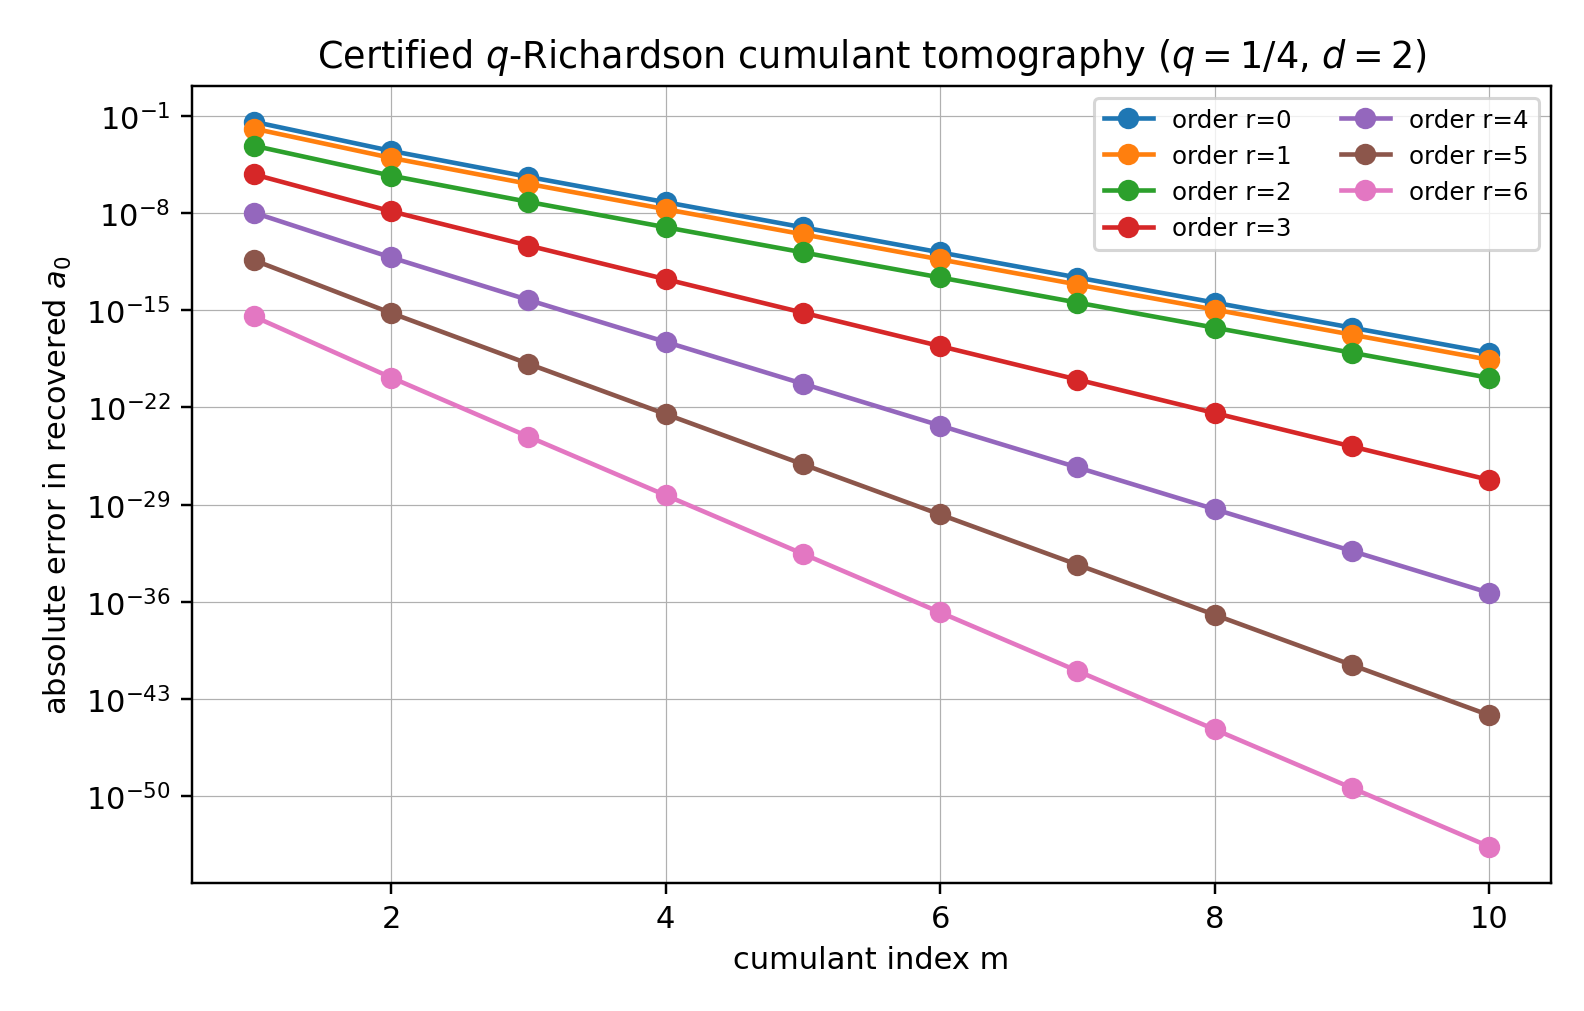
\includegraphics[width=0.91\textwidth]{figures/richardson_tomography.png}
\caption{Absolute errors in the recovery of $a_0$ from normalized cumulants
$A_2(4^{-m})$.  The CSV file retains the signs; the semilogarithmic plot shows the many
orders of magnitude gained by increasing either the cumulant index $m$ or the interpolation
order $r$.}
\label{fig:richardson}
\end{figure}

The limiting interpolation condition number was recomputed as
\[
 1.96926035366826943194719369697\ldots,
\]
in agreement with \eqref{eq:qquarter-condition}.  This is small enough that the observed
convergence reflects the exact tail annihilation rather than a cancellation between huge
floating-point weights.

\subsection{The sparse zero spectrum for $d=2$}

The generated file \path{zero_multiplicities_d2.csv} compares the prefix sum of the original
exponents with $1+\binom{\nu_2(n)}3$.  The first exceptional values are
\begin{center}
\begin{tabular}{@{}r r r@{}}
\toprule
$n$ & $\nu_2(n)$ & zero order\\
\midrule
$8$ & $3$ & $2$\\
$16$ & $4$ & $5$\\
$24$ & $3$ & $2$\\
$32$ & $5$ & $11$\\
$40$ & $3$ & $2$\\
$48$ & $4$ & $5$\\
$64$ & $6$ & $21$\\
\bottomrule
\end{tabular}
\end{center}
The spectrum is therefore classical at almost every integer but develops rapidly increasing
multiplicity on a sparse tower of highly divisible integers.

\subsection{Deterministic boundary-layer inversion}

For ranks $r=3,5,7,9$ (equivalently $d=2,4,6,8$), the script evaluates the exact truncated
characteristic product of $X_r$, inverts it on a nonaliasing FFT interval, normalizes the
resulting density, and compares its standardized CDF with the Gaussian.  The largest observed
CDF errors on $[-4,4]$ are shown in \cref{tab:boundary-errors}.

\begin{table}[htbp]
\centering
\small
\caption{Deterministic FFT check of the standardized Pascal CDF.}
\label{tab:boundary-errors}
\begin{tabular}{@{}r r r@{}}
\toprule
Rank $r$ & family degree $d=r-1$ & maximum CDF error on $[-4,4]$\\
\midrule
3 & 2 & $7.6043\times10^{-3}$\\
5 & 4 & $2.4624\times10^{-3}$\\
7 & 6 & $9.3598\times10^{-4}$\\
9 & 8 & $6.4752\times10^{-4}$\\
\bottomrule
\end{tabular}
\end{table}

\begin{figure}[htbp]
\centering
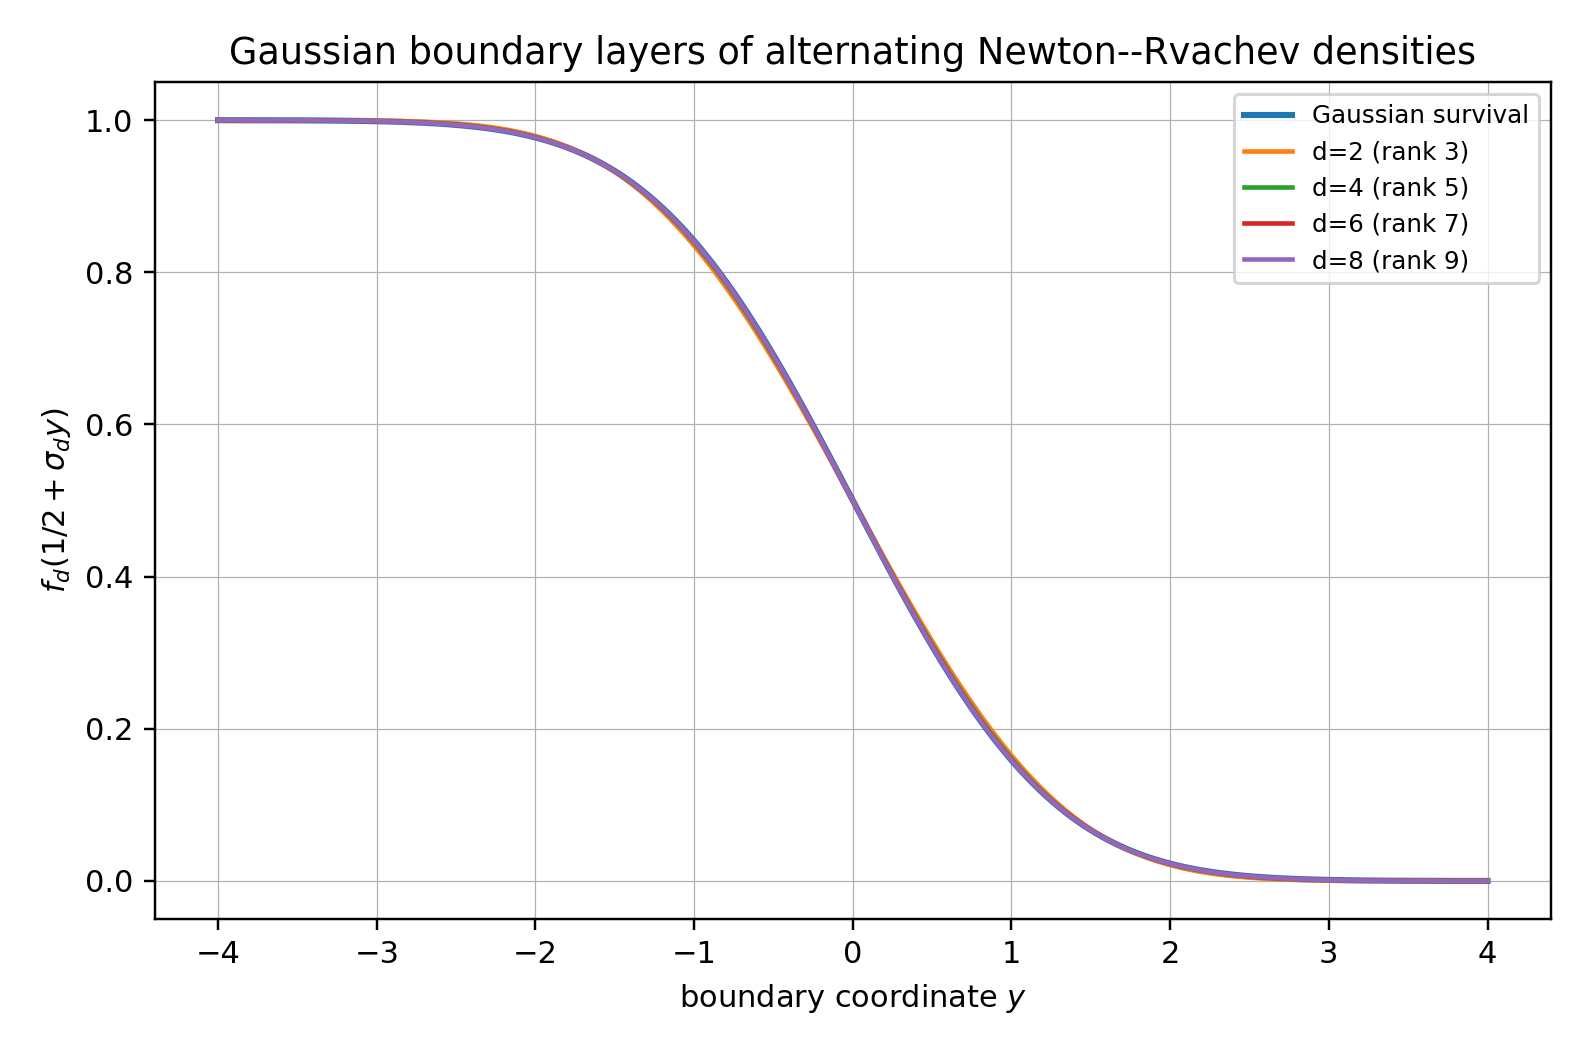
\includegraphics[width=0.91\textwidth]{figures/boundary_layers.png}
\caption{Right-edge boundary profiles
$f_d(1/2+\tau_dy)$ compared with the Gaussian survival function
$1-\NormalCDF(y)$.  The curves are obtained by deterministic Fourier inversion of the
Pascal--Rvachev characteristic products.}
\label{fig:boundary-layers}
\end{figure}

The errors decrease consistently with \cref{thm:pascal-BE}.  The theorem's universal
Berry--Esseen bound is intentionally conservative; the exact standardized fourth cumulant
\eqref{eq:pascal-standardized-k4} gives a better explanation of the observed first
correction.

\subsection{Reproduction command}

From the extracted archive, the full experiment can be rerun with
\begin{lstlisting}[style=python]
python numerical_experiments.py --output-dir reproduced-data
\end{lstlisting}
The script checks its own exact identities with assertions before writing any figure.  A
failure therefore stops the run rather than silently producing visually plausible output.


\section{Conjectures and frontier problems}
\label{sec:open}

The following statements are deliberately separated from the proved theorem package.  Each
is supported by the exact structure above, but each still requires a substantive analytic,
optimization, or arithmetic argument.

\begin{conjecture}[Uniform Edgeworth boundary expansion]
\label{conj:edgeworth}
Let $r=d+1$ and $\tau_d$ be \eqref{eq:tau-d}.  For every fixed $J$ and every fixed number of
$y$-derivatives, the two boundary profiles admit a uniform expansion
\begin{equation}
 f_d\!\left(\frac12+\tau_dy\right)
 =\NormalSurv(y)
  +\varphi(y)\sum_{j=1}^{J}E_j(y;r)
  +o\!\left((3/5)^{J(r+1)}\right),
 \label{eq:edgeworth-conj}
\end{equation}
where $\varphi$ is the Gaussian density and each $E_j$ is an explicit Hermite polynomial
whose coefficients are Bell polynomials in the standardized cumulants.  The first correction
is governed by
$\kappa_4/\sigma^4=-2(3/5)^{r+1}$.
\end{conjecture}

\paragraph{Why it is plausible.}
The triangular array has bounded summands, an entire characteristic function, and
standardized cumulants that decay exponentially with rank.  A Fourier proof should be
considerably cleaner than a generic Edgeworth theorem because the exact product provides
uniform control in both the central and large-frequency regions.

\begin{conjecture}[Minimax property of alternating $q$-tomography]
\label{conj:minimax}
Fix $q,m,r$ and the cone
\[
 \mathcal C_M=
 \left\{A(x)=\sum_{h\ge0}a_hx^h:a_h\ge0,
 \ A(q^m)\le M\right\}.
\]
Among all linear estimators using $A(q^m),\ldots,A(q^{m+r})$ and exact on polynomials of
degree at most $r$, the Lagrange estimator \eqref{eq:Rrm-def} minimizes the worst one-sided
error on $\mathcal C_M$.  Moreover, consecutive odd/even transforms form the narrowest
possible universal bracket under these constraints.
\end{conjecture}

\paragraph{Why it is plausible.}
The remainder kernel in \eqref{eq:Rrm-exact} has one sign on the coefficient cone and is the
unique kernel annihilating the first $r$ monomials.  A proof should be expressible as a
finite-dimensional linear-programming duality or a Chebyshev-system extremal argument.

\begin{conjecture}[Rational refinement transseries]
\label{conj:rational-transseries}
Let $A$ be rational, nonnegative coefficientwise, and analytic at the origin.  Then the
complete large-$t$ transseries of $\log L_a(t)$ is determined functorially by the poles of
$A$: each pole $\rho$ of order $m$ produces vertical Mellin lattices
\[
 w=\frac{\log\rho+2\pi\ii k}{\log2},
 \qquad k\in\Z,
\]
with degree-$(m-1)$ logarithmic amplitudes.  Poles on the unit circle yield bounded
log-periodic phases; poles of other moduli yield additional power scales.  No further
frequencies occur.
\end{conjecture}

\paragraph{Research route.}
Start from \eqref{eq:La-mellin}; establish a common meromorphic continuation and vertical
bounds for the rational factor, Gamma, and zeta; then shift the Mellin contour across a
finite set of pole lattices.  The main technical issue is uniform summability of the residue
series when several pole lattices have the same real part.

\begin{conjecture}[All-orders generalized inverse-Fabius expansion]
\label{conj:inverse-transseries}
For every nonnegative integer-valued polynomial $P$ of degree $d$, the endpoint CDF $G_P$ and
its inverse admit all-orders expansions in the generalized lower-Lambert coordinate
\eqref{eq:generalized-lambert}.  Their coefficients are finite differential polynomials in
the degree-$d$ periodic amplitudes of \eqref{eq:logLP-structure}; equivalently, they are
algorithmically generated from N\"orlund Bernoulli polynomials, Gamma--zeta jets, and
complete Bell polynomials.  The expansion is uniform under bounded shifts of the Lambert
phase.
\end{conjecture}

\paragraph{Why it matters.}
This would extend the corpus's inverse Fabius theory from the rank-one quadratic logarithmic
saddle to every polynomial Newton sector and would make the Lambert--Bernoulli--Bell
connection exact rather than merely formal.

\begin{problem}[The Newton positivity cone]
\label{prob:newton-cone}
Classify the integer vectors $(c_0,\ldots,c_d)$ for which
\[
 P(h)=\sum_{r=0}^{d}c_r\binom hr\ge0
 \qquad(h\in\N_0).
\]
Describe the extreme rays, the indecomposable characteristic functions
$\prod_r\Phi_{r+1}^{c_r}$, and the minimal Pascal numerator and denominator after all entire
cancellations.  Determine whether the alternating vectors
$((-1)^d,(-1)^{d-1},\ldots,1)$ for even $d$ generate distinguished extreme rays under a
natural support normalization.
\end{problem}

\begin{problem}[Arithmetic of generalized half-integer spectra]
For a rational generating function $A$ with integer coefficients, classify the fields,
traces, and norms of
\[
 \Phi_a\!\left(k+\frac12\right).
\]
The audited half-integer report handles the classical exponent sequence.  The master
zero/cumulant dictionary suggests that rational $A$ should produce finite-dimensional
cyclotomic trace recurrences, but the orders and positivity constraints will depend on the
pole data of $A$.
\end{problem}

\begin{problem}[Optimal smooth approximation of the box within the Newton family]
At fixed support and fixed highest Newton degree, choose a nonnegative integer-valued
polynomial $P$ to minimize one of
\[
 \|f_P-b\|_1,
 \qquad
 W_2(\Law(X_P),\Law(U)),
 \qquad
 \sup_{|\xi|\le T}|\Phi_P(\xi)-\sinc(\xi)|.
\]
The family $P_d(h)=\binom{h-1}{d}$ is natural because it appends one rescaled Pascal law to a
box, but it is not yet known to be extremal under any of these criteria.
\end{problem}


\section{Formalization and computational research program}
\label{sec:formalization}

The theorem package is unusually suitable for staged Lean formalization: its algebraic core
is finite, and the analytic results can be added only after the exact identities are stable.
A dependency-aware order is as follows.

\subsection{Phase I: finite algebra and digital combinatorics}

\begin{enumerate}
\item Define exponent prefixes and prove
      $m_a(n)=\sum_{h\le\nu_2(n)}a_h$ for finite products.
\item Prove the finite zero-count identity
      $M_a(N)=\sum_ha_h\lfloor N/2^h\rfloor$ and the binary defect
      \eqref{eq:M-bit}.
\item Define the generalized sign character and prove
      \eqref{eq:kernel-shift}; formalize the automaticity equivalence for eventually
      periodic parity words.
\item Prove the finite sign-product factorization \eqref{eq:T-a-L}, its exact order at one,
      and the first surviving moment \eqref{eq:first-surviving}.
\item Reuse the compiled geometric Lagrange weights, Gaussian-binomial closed form,
      principal specialization, and exact survivor; then formalize the still-open
      sign-certified Richardson remainder.
\end{enumerate}

These statements require only finite sums, polynomials, valuations, and existing
$q$-binomial infrastructure.

\subsection{Phase II: probability and entire products}

\begin{enumerate}
\item Construct $X_a$ from finite uniform sums and pass to the bounded infinite series using
      the summability hypothesis $A(1/2)<\infty$.
\item Prove local uniform convergence of $\Phi_a$ and the convolution-monoid law.
\item Derive cumulants from the uniform Bernoulli expansion and moments from the existing
      Bell-polynomial library.
\item Formalize identifiability first from zero multiplicities, then from analytic samples
      $A(4^{-j})$.
\item Build polynomial exponent sequences from Newton expansions and prove the entire
      cancellation behind \eqref{eq:newton-Phi-factorization}.
\end{enumerate}

\subsection{Phase III: asymptotics and inverse functions}

\begin{enumerate}
\item Reuse the corpus's Mellin kernel theorem to prove \eqref{eq:La-mellin} for polynomial
      weights.
\item Formalize pole orders and the leading coefficient $C_P$ before attempting the full
      periodic residue expansion.
\item Transfer the existing Pascal-hierarchy Fourier envelope to a general polynomial by
      the Newton factorization and lower-order comparison.
\item Prove the leading small-ball and inverse laws using the already formalized exponential
      Tauberian infrastructure, or isolate that theorem as a reusable library component.
\item Only then lift the classical all-orders saddle and inverse-Lambert machinery to the
      higher-order pole hierarchy.
\end{enumerate}

\subsection{Certified computation}

The tomography algorithm is a natural application for exact rationals and interval
arithmetic.  At $q=1/4$ all Lagrange weights are rational, as are the normalized cumulants of
integer exponent sequences.  A verified executable can therefore recover coefficients with
no floating-point assumptions.  For asymptotic experiments, Arb-style ball arithmetic would
certify Mellin residues, Lambert branches, and boundary-layer errors.  The supplied Python
script is a reproducible exploratory implementation, not a substitute for that final
certification layer.


\section{Conclusion}
\label{sec:conclusion}

The central result of this report is a change of viewpoint.  Instead of treating the
classical Rvachev transform, the Pascal hierarchy, its zero spectrum, its cumulants, and its
endpoint asymptotics as separate constructions, one begins with the exponent generating
function
\[
 A(q)=\sum_{h\ge0}a_hq^h.
\]
The same $A$ then appears at four geometrically related arguments:
\begin{equation}
 \begin{array}{ccl}
 A(1/2) &:& \text{support radius},\\
 A(2^{-s}) &:& \text{spectral zeta and zero divisor},\\
 A(4^{-j}) &:& \text{even cumulants},\\
 A(2^w) &:& \text{endpoint Mellin transform}.
 \end{array}
 \label{eq:four-samples-summary}
\end{equation}
Its coefficient parity is the Fourier-lobe character, its prefix sums are zero
multiplicities, its rationality is finite refinement rank, and its Newton coordinates are
Pascal--Rvachev exponents.

Three consequences seem especially durable.

First, the spectral and probabilistic data are identifiable: the zero divisor or the full
even-cumulant sequence determines the hidden dyadic convolution law.  The
Gaussian-$q$-binomial Richardson transform makes that statement constructive and supplies
certified alternating bounds.

Second, nonnegative integer-valued polynomials form a rich positive-definite quotient sector.
Negative Pascal exponents are not pathologies when they recombine into a nonnegative scale
sequence.  The family
$P_d(h)=\binom{h-1}{d}$ gives the explicit quotient
$\Phi_1\Phi_3/\Phi_2$ at $d=2$, sparse enhanced zero divisors, automatic lobe signs, and a
smooth approximation to the box with an exact Gaussian edge profile.

Third, Mellin reflection makes the endpoint and spectrum literally the same meromorphic
object viewed at $s$ and $-s$.  Polynomial degree becomes pole order; pole order becomes the
power of the endpoint logarithm; the dyadic pole lattice becomes the periodic coefficient
hierarchy; and the leading saddle is solved by a generalized lower branch of Lambert $W$.
N\"orlund Bernoulli polynomials and complete Bell polynomials then supply the coefficient
algebra required for an all-orders inverse theory.

These deductions are new relative to the pinned 67-source corpus, but they are not presented
as the end of the subject.  Their main value is that they turn a collection of striking
special identities into a classification problem with exact algebraic coordinates, stable
reconstruction algorithms, and a clear route to formal verification.

\appendix
\section{Complete recursive corpus inventory}
\label{app:inventory}

The following path ledger is the authoritative source list used for the nonduplication audit.
Every path is relative to \path{Analysis/FabiusFunction/docs/}.  The pinned commit is
\texttt{32d6d36c51d803289e6d6a0dc0c37753766eba47}.  The count is 67.  Frozen revisions were
read for distinctive claims and provenance, but a repeated theorem in several revisions was
counted once when determining novelty.

{\small
\begin{longtable}{@{}r >{\raggedright\arraybackslash}p{0.88\textwidth}@{}}
\toprule
No. & Relative path\\
\midrule
\endfirsthead
\multicolumn{2}{c}{\small\itshape Corpus inventory (continued)}\\[0.3em]
\toprule
No. & Relative path\\
\midrule
\endhead
\midrule
\multicolumn{2}{r}{\small\itshape Continued on the next page}\\
\endfoot
\bottomrule
\endlastfoot
1 & \path{FabiusFunction_Mathematical_Glossary/FabiusFunction_Mathematical_Glossary.tex}\\
2 & \path{Fabius_Function_and_Rvachev_Up/Fabius_Function_and_Rvachev_Up.tex}\\
3 & \path{Non_Elementarity_of_the_Fabius_Function/Non_Elementarity_of_the_Fabius_Function.tex}\\
4 & \path{fabius_lean_walkthrough/fabius_lean_walkthrough.tex}\\
5 & \path{non-formalized-research-frontiers/non-formalized-research-frontiers.tex}\\
6 & \path{archive/early-notes/Fabius Asymptotic/Fabius Asymptotic.tex}\\
7 & \path{archive/early-notes/K-fold summation over the signed Thue-Morse sequence/K-fold summation over the signed Thue-Morse sequence.tex}\\
8 & \path{archive/glossary/FabiusFunction_Mathematical_Glossary-2/FabiusFunction_Mathematical_Glossary.tex}\\
9 & \path{archive/glossary/FabiusFunction_Mathematical_Glossary/FabiusFunction_Mathematical_Glossary.tex}\\
10 & \path{archive/lean-walkthrough/Fabius_Function_Lean_Walkthrough/Fabius_Function_Lean_Walkthrough.tex}\\
11 & \path{archive/lean-walkthrough/fabius_lean_walkthrough/fabius_lean_walkthrough.tex}\\
12 & \path{archive/primary-exposition/Fabius_Function_and_Rvachev_Up-2/Fabius_Function_and_Rvachev_Up.tex}\\
13 & \path{archive/primary-exposition/Fabius_Function_and_Rvachev_Up-3/Fabius_Function_and_Rvachev_Up.tex}\\
14 & \path{archive/primary-exposition/Fabius_Function_and_Rvachev_Up/Fabius_Function_and_Rvachev_Up.tex}\\
15 & \path{archive/primary-exposition/Fabius_and_Rvachev_Up-2/Fabius_and_Rvachev_Up.tex}\\
16 & \path{archive/primary-exposition/Fabius_and_Rvachev_up/Fabius_and_Rvachev_up.tex}\\
17 & \path{archive/primary-exposition/Fabius_function_and_up_function/Fabius_function_and_up_function.tex}\\
18 & \path{archive/primary-supplements/Fabius_Function_Missing_Parts-2/Fabius_Function_Missing_Parts.tex}\\
19 & \path{archive/primary-supplements/Fabius_Function_Missing_Parts/Fabius_Function_Missing_Parts.tex}\\
20 & \path{archive/q-calculus/Fabius_q_Special_Functions/Fabius_q_Special_Functions.tex}\\
21 & \path{archive/q-calculus/fabius-q-special-functions/fabius-q-special-functions.tex}\\
22 & \path{archive/research-frontiers/Fabius_Dyadic_Asymptotic_Bridge/Fabius_Dyadic_Asymptotic_Bridge.tex}\\
23 & \path{archive/research-frontiers/Fabius_Dyadic_Formulae_and_Alternative_Representations/Fabius_Dyadic_Formulae_and_Alternative_Representations.tex}\\
24 & \path{archive/research-frontiers/Fabius_Dyadic_Formulae_to_Asymptotics/Fabius_Dyadic_Formulae_to_Asymptotics.tex}\\
25 & \path{archive/research-frontiers/Fabius_Dyadic_q_Connections/Fabius_Dyadic_q_Connections.tex}\\
26 & \path{archive/research-frontiers/Fabius_Thue_Morse_Convergence_Rate/Fabius_Thue_Morse_Convergence_Rate.tex}\\
27 & \path{archive/research-frontiers/Fabius_Thue_Morse_Convergence_Rates/Fabius_Thue_Morse_Convergence_Rates.tex}\\
28 & \path{archive/research-frontiers/Primary_Exposition_Gap_Register/Primary_Exposition_Gap_Register.tex}\\
29 & \path{archive/research-frontiers/Repeated_Integration_and_Rvachev_Up/Repeated_Integration_and_Rvachev_Up.tex}\\
30 & \path{archive/research-frontiers/Rvachev_Up_from_Repeated_Integration/Rvachev_Up_from_Repeated_Integration.tex}\\
31 & \path{archive/research-frontiers/Thue_Morse_Formula_Atlas-1/Thue_Morse_Formula_Atlas.tex}\\
32 & \path{archive/research-frontiers/Thue_Morse_Formula_Atlas-2/Consolidated_Formula_Atlas_for_the_Thue_Morse_Sequence.tex}\\
33 & \path{archive/research-frontiers/Thue_Morse_Formula_Atlas-3/Thue_Morse_Formula_Atlas.tex}\\
34 & \path{archive/research-frontiers/non-formalized-research-frontiers/non-formalized-research-frontiers.tex}\\
35 & \path{archive/standalone-studies/Non_Elementarity_of_the_Fabius_Function/Non_Elementarity_of_the_Fabius_Function.tex}\\
36 & \path{archive/standalone-studies/Small_Argument_Asymptotics/Small_Argument_Asymptotics.tex}\\
37 & \path{archive/standalone-studies/fabius-inverse-dyadic-closed-form/fabius-inverse-dyadic-closed-form.tex}\\
38 & \path{non-formalized-research-frontiers/drafts/Fabius_Arithmetic_Rays_Frontier_Report/Fabius_Arithmetic_Rays_Frontier_Report.tex}\\
39 & \path{non-formalized-research-frontiers/drafts/Fabius_Half_Integer_Spectral_Frontier_Report/Fabius_Half_Integer_Spectral_Frontier_Report.tex}\\
40 & \path{non-formalized-research-frontiers/drafts/Fabius_Rvachev_Frontier_Report-2/Fabius_Rvachev_Frontier_Report.tex}\\
41 & \path{non-formalized-research-frontiers/drafts/Fabius_Rvachev_Frontier_Report/Fabius_Rvachev_Frontier_Report.tex}\\
42 & \path{non-formalized-research-frontiers/drafts/Fabius_Rvachev_New_Frontiers/Fabius_Rvachev_New_Frontiers.tex}\\
43 & \path{non-formalized-research-frontiers/drafts/Fabius_Rvachev_Thue_Morse_Frontier_Results/Fabius_Rvachev_Thue_Morse_Frontier_Results.tex}\\
44 & \path{non-formalized-research-frontiers/drafts/Spectral_Arithmetic_Pascal_Rvachev_Hierarchy/Spectral_Arithmetic_Pascal_Rvachev_Hierarchy.tex}\\
45 & \path{non-formalized-research-frontiers/drafts/Thue_Morse_Formula_Atlas/Thue_Morse_Formula_Atlas.tex}\\
46 & \path{non-formalized-research-frontiers/drafts/fabius_frontier_new_results/fabius_frontier_new_results.tex}\\
47 & \path{non-formalized-research-frontiers/drafts/fabius_frontier_results_bundle/fabius_frontier_results.tex}\\
48 & \path{non-formalized-research-frontiers/drafts/fabius_frontier_spectral_endpoint_report_bundle/fabius_frontier_spectral_endpoint_report.tex}\\
49 & \path{non-formalized-research-frontiers/drafts/rvachev_up_fourier_decay/Rvachev_Up_Fourier_Decay-2/Rvachev_Up_Fourier_Decay.tex}\\
50 & \path{non-formalized-research-frontiers/drafts/rvachev_up_fourier_decay/Rvachev_Up_Fourier_Decay-3/Fourier_decay_of_Rvachev_up.tex}\\
51 & \path{non-formalized-research-frontiers/drafts/rvachev_up_fourier_decay/Rvachev_Up_Fourier_Decay_Comparative_Audit/Rvachev_Up_Fourier_Decay_Comparative_Audit.tex}\\
52 & \path{non-formalized-research-frontiers/drafts/rvachev_up_fourier_decay/Rvachev_Up_Fourier_Decay_Gentle_Guide/Rvachev_Up_Fourier_Decay_Gentle_Guide.tex}\\
53 & \path{non-formalized-research-frontiers/drafts/rvachev_up_fourier_decay/Rvachev_Up_Fourier_Decay_Second_Wave_Audit/Rvachev_Up_Fourier_Decay_Second_Wave_Audit.tex}\\
54 & \path{non-formalized-research-frontiers/drafts/rvachev_up_fourier_decay/asymptotic-decay-rate-of-an-infinite-product-of-sinc-functions/asymptotic-decay-rate-of-an-infinite-product-of-sinc-functions.tex}\\
55 & \path{non-formalized-research-frontiers/drafts/rvachev_up_fourier_decay/rvachev_up_fourier_decay-1/rvachev_up_fourier_decay.tex}\\
56 & \path{non-formalized-research-frontiers/drafts/rvachev_up_fourier_decay/rvachev_up_fourier_decay-4/rvachev_up_fourier_decay.tex}\\
57 & \path{non-formalized-research-frontiers/drafts/rvachev_up_fourier_decay/rvachev_up_fourier_decay-5/Rvachev_Up_Fourier_Decay_Final.tex}\\
58 & \path{non-formalized-research-frontiers/drafts/rvachev_up_fourier_decay/rvachev_up_fourier_decay-6/Rvachev_Up_Fourier_Decay_Final_Synthesis.tex}\\
59 & \path{non-formalized-research-frontiers/drafts/rvachev_up_fourier_decay/rvachev_up_fourier_decay-7/rvachev_up_fourier_decay_final.tex}\\
60 & \path{non-formalized-research-frontiers/drafts/rvachev_up_fourier_decay/rvachev_up_fourier_decay-8/rvachev_up_fourier_decay_final.tex}\\
61 & \path{papers/AIF_2017__67_2_637_0/AIF_2017__67_2_637_0-corrected.tex}\\
62 & \path{papers/AIF_2017__67_2_637_0/AIF_2017__67_2_637_0.tex}\\
63 & \path{papers/arXiv-1502.06738v2/Lacunary_products.tex}\\
64 & \path{papers/arXiv-1702.05442v1/09-Function.tex}\\
65 & \path{papers/arXiv-1702.06487v3/157-Arithmetic-v3.tex}\\
66 & \path{papers/arXiv-2211.13570v1/document.tex}\\
67 & \path{papers/ubiq15/ubiq15-corrected.tex}\\
\end{longtable}
}


\section{Result ledger and dependency map}
\label{app:ledger}

\Cref{tab:result-ledger} records the logical status and principal inputs of the report's main
claims.  It is intended to make later formalization and peer checking easier: a reader can
separate finite algebra from analytic continuation, and new deductions from imported
frontier theorems.

\begin{longtable}{@{}>{\raggedright\arraybackslash}p{0.08\textwidth}>{\raggedright\arraybackslash}p{0.42\textwidth}>{\raggedright\arraybackslash}p{0.16\textwidth}>{\raggedright\arraybackslash}p{0.25\textwidth}@{}}
\caption{Result and proof-dependency ledger.}
\label{tab:result-ledger}\\
\toprule
ID & Statement & Status & Main inputs\\
\midrule
\endfirsthead
\toprule
ID & Statement & Status & Main inputs\\
\midrule
\endhead
A1 & Exponent-sequence probability law, support, entire product, convolution monoid & proved & uniform characteristic function; normal convergence\\
A2 & Zero multiplicity $m_a(n)$ and zeta $\zeta(s)A(2^{-s})$ & proved & Euler product; Tonelli/rearrangement\\
A3 & Digital zero defect and generalized lobe character & proved & binary floors; parity\\
A4 & Automaticity iff the parity word is eventually periodic & proved & exact $2$-kernel/shift identity\\
A5 & General Prouhet order and first surviving power moment & proved & finite product; falling factorials\\
B1 & Cumulant transform $B_{2j}A(4^{-j})/(2j)$ & proved & uniform cumulants; additivity\\
B2 & Identifiability from zeros, zeta, or all even cumulants & proved & prefix differences; identity theorem\\
B3 & Gaussian-$q$-binomial tomography and one-sided remainder & proved & Lagrange interpolation; principal specialization\\
B4 & Bounded exact condition number $(-q;q)_r/(q;q)_r$ & proved & finite $q$-binomial theorem\\
C1 & Shift/refinement identity and rational finite-rank classification & proved & reindexing; rational-series theorem\\
C2 & Newton factorization of nonnegative polynomial weights & proved & integer-valued polynomial calculus\\
C3 & Leading Fourier, small-ball, and inverse laws & derived & audited Pascal hierarchy; de Bruijn transfer\\
D1 & Alternating family $P_d(h)=\binom{h-1}{d}$ and positive quotient & proved & Newton identity; random-series factorization\\
D2 & Sparse spectrum, exact cumulants, automatic Prouhet selector & proved & hockey-stick; Lucas theorem\\
D3 & Gaussian edge layer, exact $L^1$ law, TV and $W_2$ bounds & proved & Berry--Esseen; interval overlap\\
E1 & Mellin reflection between endpoint Laplace and spectral zeta & proved & Mellin kernel; geometric scaling\\
E2 & Polynomial/log-periodic pole hierarchy & proved structurally & Mellin residues; rational pole orders\\
E3 & All-orders generalized inverse transseries & conjectural & uniform higher-pole saddle analysis needed\\
\bottomrule
\end{longtable}

\section{Reproducibility manifest}
\label{app:manifest}

The companion archive contains:
\begin{center}
\begin{tabularx}{0.96\textwidth}{@{}p{0.34\textwidth}X@{}}
\toprule
Path & Purpose\\
\midrule
\path{Exponent_Sequence_Newton_Rvachev_Frontiers.tex} & Complete manuscript source.\\
\path{Exponent_Sequence_Newton_Rvachev_Frontiers.pdf} & Rendered report.\\
\path{numerical_experiments.py} & Commented high-precision and FFT verification program.\\
\path{figures/richardson_tomography.png} & Figure used in \cref{fig:richardson}.\\
\path{figures/boundary_layers.png} & Figure used in \cref{fig:boundary-layers}.\\
\path{data/richardson_tomography.csv} & Full signed extrapolation errors.\\
\path{data/boundary_layer_errors.csv} & Deterministic standardized-CDF errors.\\
\path{data/zero_multiplicities_d2.csv} & Direct and closed-form zero orders for the $d=2$ family.\\
\path{data/verification_log.txt} & Precision settings, assertion status, and headline values.\\
\path{README.md} & Build and reproduction commands.\\
\path{requirements.txt} & Exact Python package versions used for the numerical audit.\\
\path{SHA256SUMS} & Checksums for the report, code, figures, and data.\\
\bottomrule
\end{tabularx}
\end{center}

The numerical script fixes the precision and grid sizes explicitly.  Its formulas use
\texttt{numpy.sinc(x)}=$\sin(\pi x)/(\pi x)$, matching the normalization in
\eqref{eq:sinc-normalized}.  The FFT interval is wider than the compact support, so periodic
copies do not overlap.  All exact checks run before figure generation.


\begin{thebibliography}{99}

\bibitem{aistleitner2015}
C.~Aistleitner, R.~Hofer, and G.~Larcher,
\emph{On parametric Thue--Morse sequences and lacunary trigonometric products},
arXiv:1502.06738v2, 2015.

\bibitem{alloucheShallit}
J.-P.~Allouche and J.~Shallit,
\emph{Automatic Sequences: Theory, Applications, Generalizations},
Cambridge University Press, 2003.

\bibitem{andrews1976}
G.~E.~Andrews,
\emph{The Theory of Partitions},
Encyclopedia of Mathematics and its Applications, Vol.~2,
Addison--Wesley, 1976; reprinted by Cambridge University Press.

\bibitem{arias1982}
J.~Arias de Reyna,
\emph{An infinitely differentiable function with compact support: definition and
properties}, Rev. Real Acad. Ciencias Madrid \textbf{76} (1982), 21--38;
English translation, arXiv:1702.05442, 2017.

\bibitem{arias2017}
J.~Arias de Reyna,
\emph{Arithmetic of the Fabius function},
Ann. Inst. Fourier (Grenoble) \textbf{67} (2017), no.~2, 637--679;
arXiv:1702.06487v3.

\bibitem{corless1996}
R.~M.~Corless, G.~H.~Gonnet, D.~E.~G.~Hare, D.~J.~Jeffrey, and D.~E.~Knuth,
\emph{On the Lambert $W$ function},
Adv. Comput. Math. \textbf{5} (1996), 329--359.

\bibitem{debruijn1959}
N.~G.~de Bruijn,
\emph{Pairs of slowly oscillating functions occurring in asymptotic problems concerning
the Laplace transform},
Nieuw Arch. Wisk. (3) \textbf{7} (1959), 20--26.

\bibitem{flajolet1995}
P.~Flajolet, X.~Gourdon, and P.~Dumas,
\emph{Mellin transforms and asymptotics: harmonic sums},
Theoret. Comput. Sci. \textbf{144} (1995), 3--58.

\bibitem{norlund1924}
N.~E.~N\"orlund,
\emph{Vorlesungen \"uber Differenzenrechnung},
Grundlehren der mathematischen Wissenschaften, Vol.~13,
Springer, Berlin, 1924.

\bibitem{petrov1995}
V.~V.~Petrov,
\emph{Limit Theorems of Probability Theory: Sequences of Independent Random Variables},
Oxford Studies in Probability, Vol.~4, Clarendon Press, Oxford, 1995.

\bibitem{stanley1997}
R.~P.~Stanley,
\emph{Enumerative Combinatorics, Vol.~1}, second printing,
Cambridge Studies in Advanced Mathematics, Vol.~49,
Cambridge University Press, 1997.

\bibitem{toth2022}
L.~T\'oth,
\emph{Linear combinations of Dirichlet series associated with the Thue--Morse sequence},
Integers \textbf{22} (2022), Paper A98; arXiv:2211.13570.

\bibitem{voss2009}
J.~Voss,
\emph{Upper and lower bounds in exponential Tauberian theorems},
Tbilisi Math. J. \textbf{2} (2009), 41--50; arXiv:0908.0642.

\bibitem{proveit}
V.~Reshetnikov,
\emph{ProveIt: formal and expository development of the Fabius function},
GitHub repository, pinned in this report at commit
\texttt{32d6d36c51d803289e6d6a0dc0c37753766eba47}, 27 August 2026.

\end{thebibliography}

\end{document}
